% Created 2024-03-15 Fri 12:47
% Intended LaTeX compiler: pdflatex
\documentclass[ee,proposal]{usuthesis}
\usepackage[utf8]{inputenc}
\usepackage[T1]{fontenc}
\usepackage{graphicx}
\usepackage{longtable}
\usepackage{wrapfig}
\usepackage{rotating}
\usepackage[normalem]{ulem}
\usepackage{amsmath}
\usepackage{amssymb}
\usepackage{capt-of}
\usepackage{hyperref}
\usepackage{amsmath}                         % Miscellaneous enhancements for mathematics
\usepackage{amssymb}                         % Math symbols
\usepackage{algorithm2e}                    % Algorithms
\usepackage{amsfonts}                       % Cool math fonts
\usepackage{booktabs}                       % Used for lines in table
\usepackage{lipsum}                         % Dummy filler text
\usepackage{multicol}                       % Add capability to make columns
\usepackage{multirow}                       % Add capability to make rows
\usepackage{pgfgantt}                       % Add capability to create gantt charts
\usepackage{standalone}                     % Allow standalone documents
\usepackage{subcaption}                     % Allow subfigures
\usepackage{subfloat}                       % Subfigures
\usepackage{tabularx}                        % Add more contol to tables
\usepackage{listings}                       % Display code
\usepackage{doi}                            % Hyperling DOI
\usepackage{hyperref}                       % Cool clean hyperlinks
\hypersetup{colorlinks=true, linkcolor=blue,
citecolor=blue,urlcolor=blue} % Use when compiling the digital copy
\usetikzlibrary{arrows.meta}                % Arrows for tikz
\renewcommand*{\chapterautorefname}{Chapter}
\renewcommand*{\sectionautorefname}{Section}
\renewcommand*{\subsectionautorefname}{Subsection}
\renewcommand*{\subsubsectionautorefname}{Subsubsection}
\renewcommand*{\paragraphautorefname}{Paragraph}
\renewcommand*{\algorithmautorefname}{Algorithm}
\newcommand{\definitionautorefname}{Definition}
\newcommand{\Or}{\textbf{ or }}
\renewcommand*{\And}{\textbf{ and }}
\newcommand\mycommfont[1]{\footnotesize\ttfamily\textcolor{gray}{#1}}
\newcommand{\T}{\mathcal{T}}                % To make it clear the difference
\newcommand{\Tau}{T}                        % between Tau and T
\newcommand{\AC}{AC(u, d, v, \eta)}            % Set the parameters for AC once
\newcommand{\PC}{PC(u, d, v)}               % Set the parameters for PC once
\newcommand{\ACi}{AC(u_i, d_i, v_i, \eta_i)}% Set the parameters for AC once
\newcommand{\PCi}{PC(u_i, d_i, v_i)}        % Set the parameters for PC once
\newcommand{\Not}{\textbf{not }}            % Custom `not' operator
\newcommand{\visit}{(b_i, a_i, e_i, u_i, d_i, v_i, \eta_i, \xi_i)}
\newcommand{\I}{\mathbb{I}}                 % Set of visit tuples
\newcommand{\C}{\mathbb{C}}                 % Charger availability information
\newcommand{\U}{\mathcal{U}}                % Uniform distribution
\newcommand{\W}{\mathcal{W}}                % Weighted distribution
\newcommand{\Sol}{\mathbb{S}}               % A shorthand for visit tuple
\newcommand{\M}{\mathbb{M}}                 % A shorthand for the metadata
\newcommand{\Hd}{\mathbb{H}}                % Set of discrete times
\newcommand{\Nu}{\mathcal{V}}               % Draw a nice Nu
\newcommand{\Iset}{I}                       % Set of visits 1-I
\newcommand{\Isetinit}{I_0}                 % Set of visits inital visits
\newcommand{\Isetfinal}{I_f}                % Set of visits final visits
\newcommand{\Bset}{B}                       % Set of visits 1-B
\newcommand{\Qset}{Q}                       % Set of visits 1-Q
\newcommand{\Jset}{J}                       % Set of visits 1-J
\newcommand{\Jsetq}{\mathbb{J}}             % Set of visits 1-J for queue active times
\newcommand{\Hset}{H}                       % Set of visits 1-H
% The Committee
\majorprof{Dr. Greg Droge, Ph.D.}
\firstreader{Dr. Jacob Gunther, Ph.D.}
\secondreader{Dr. Burak Sarsilmaz, Ph.D.}


% Degree Information
\degree{Master of Science}
\month{Dec}
\gradyear{2024}
\newtheorem{definition}{Definition}[section]
\author{Alexander Brown}
\date{}
\title{The Simulated Annealing Fully Fuzzy Position Allocation Problem Utilizing Mixed Integer Linear Programming Constraints with Non-Linear Battery Dynamics}
\hypersetup{
 pdfauthor={Alexander Brown},
 pdftitle={The Simulated Annealing Fully Fuzzy Position Allocation Problem Utilizing Mixed Integer Linear Programming Constraints with Non-Linear Battery Dynamics},
 pdfkeywords={},
 pdfsubject={},
 pdfcreator={Emacs 29.2 (Org mode 9.6.15)}, 
 pdflang={English}}
\begin{document}

\let\ref\autoref                            % Redifine `\ref` as `\autoref` because lazy
\SetCommentSty{mycommfont}                  % Set the comment color

\preliminaries   % set frontmatter style

\maketitle

\tableofcontents
\listoftables
\listoffigures

\body  % set main body style

\chapter{INTRODUCTION}
\label{sec:introduction}
Public transportation systems are crucial in any urban area; however, the increased awareness and concern of
environmental impacts of petroleum based public transportation has driven an effort to reduce the pollutant footprint
\cite{de-2014-simul-elect,xylia-2018-role-charg,guida-2017-zeeus-repor-europ,li-2016-batter-elect}. Particularly,
the electrification of public bus transportation via battery power, i.e., battery electric buses (BEBs), has received
significant attention \cite{li-2016-batter-elect}. Although the technology provides benefits beyond reduction in
emissions, such as lower driving costs, lower maintenance costs, and reduced vehicle noise, battery powered systems
introduce new challenges such as larger upfront costs, and potentially several hours long ``refueling'' periods
\cite{xylia-2018-role-charg,li-2016-batter-elect}. Furthermore, the problem is exacerbated by the constraints of the
transit schedule to which the fleet must adhere, the limited amount of chargers available, and the adverse affects in
the health of the battery due to fast charging \cite{lutsey-2019-updat-elect}.

BEBs have been in service for many major markets, North America, Europe, and China, for more than a decade with expected
growth in the near future \cite{deng-2021-survey-elect}. The Asia Pacific market is forecasted to dominate the sales
and some major companies of the industry have also begun to enter the global market such as Volvo, BYD, and Proterra by
2025 \cite{deng-2021-survey-elect}. Much focus has been placed on the engineering of individual BEBs such as battery
type, brake regenerative charging, optimal battery charging, and battery degradation \cite{chen-2008-desig-grey,abdollahi-2016-optim-batter,kuhne-2010-elect,deng-2021-survey-elect}. The interest of route scheduling, charging
fleets, and optimizing the infrastructure are problems of more recent interest and are therefore timely and increasingly
relevant problems as EV/BEBs become more commonplace \cite{hoke-2014-accoun-lithium,sebastiani-2016-evaluat-elect,wei-2018-optim-spatio}.

The literature shows an interest in solving the problem of assigning BEBs to charging queues or optimizing their
infrastructure \cite{wei-2018-optim-spatio,sebastiani-2016-evaluat-elect,hoke-2014-accoun-lithium,wang-2017-elect-vehic}. In fact, many works attempt to solve both problems simultanously
barring some simplification whether it be only allowing chargers of a single type
\cite{he-2020-optim-charg,tang-2019-robus-sched}. If multiple chargers are used, then one of each type is assigned at
each location. Others have also assumed that a BEB shall recieve full charge upon each arrival
\cite{wei-2018-optim-spatio,wang-2017-elect-vehic,zhou-2020-bi-objec,wang-2017-optim-rechar}. Some works on the
stochastic effects of energy consumption while on route for a BEB as well as trip times \cite{zhou-2020-collab-optim,bie-2021-optim-elect}. One other source, as far as the reseach for this work has shown, describes a method of producing
a BEB charge schedule wih a high fidelity while accounting for multiple charger times as well as being able to minimize
over the total charger count \cite{whitaker-2023-a-network}.

The work described in this proposal is similar to the work in \cite{whitaker-2023-a-network}; however provides an
alternate method of modeling the problem in what is known as the Position Allocation Problem (PAP). The PAP is modeled
after the Berth Allocation Problem (BAP), which was designed to optimally schedule cargo vessels to be berthed and
serviced \cite{buhrkal-2011-model-discr,imai-2001-dynam-berth,frojan-2015-contin-berth}. The PAP utilizes this
notion to develop a model of assigning EVs to queue in ordered to be charged \cite{qarebagh-2019-optim-sched}.

Because of the PAP's extremely close modeling methods to the BAP, literature from the BAP can (and will) provide support
for the development of the PAP in this work. The BAP has been studied in literature since the 1990s and provides a depth
of work to derive from \cite{rodrigues-2022-berth}. The work to be introduced promises much potential for further
research and development in regard to scheduling BEBs. What follows is a proposal for a Simulated Annealing (SA)
implementation and extension of the PAP utilizing Mixed Integer Linear Programming (MILP) constraints with non-linear
battery dynamics.

In the next section, a review of relevant literature of BEBs is introduced and discussed. Background and a problem
statement will be elaborated further to provide context and a required basis of understanding prior to discussing the
objectives and approaches in \ref{sec:objectives} and \ref{sec:approach}, respectively. The BEB queue scheduling problem discussed
throughout this section is of particular interest at this time in the BEB industry and requires more attention. The
research proposed directly approaches this problem by improving upon existing implementations to provide a robust and
accurate solution. In the subsequent sections the objectives will be introduced in \ref{sec:objectives} and the approach for
each objective will be discussed in \ref{sec:approach}.
\chapter{OBJECTIVES}
\label{sec:objectives}
The field of BEB research provides exciting many avenues and is continuing to gain traction in industry as BEBs replace
their gasoline counterparts. This work will introduce a novel approach to BEB scheduling that minimizes monetary costs
for the user, provides a robust solution, and includes an accurate dynamic battery model. The PAP provides a solid
foundation from which this work derived. However, the PAP does not perfectly encapsulate the problem and thus needs some
modifications to accommodate the BEB model. The PAP does not account for the revisits of a BEB and therefore the
State-Of-Charge (SOC) cannot be tracked. The model does not account for multiple charger types, and in fact models the
charger as a single continuous bar. These accommodations must be accounted for and are included in the objectives for
the proposed BEB charging plan below.

\begin{itemize}
\item \textbf{Objective 1}: Mathematically model the PAP to optimally assign BEBs to queues with unknown charging times to allow consideration of consumption cost and battery health

\begin{itemize}
\item \textbf{Task 1.1}: Modify PAP to enable multiple visits by a BEB with variable charger duration per visit.

\item \textbf{Task 1.2}: Incorporate heterogeneous charger capabilities into the PAP to model slow and fast charging, minimize
and total charger count. Slow charging will be incentivized for battery health and consumption cost.
\end{itemize}

\item \textbf{Objective 2}: Develop robust charger allocation capabilities to account for non-linear battery dynamics

\begin{itemize}
\item \textbf{Task 2.1}: Incorporate non-linear battery dynamics into the FFLP PAP model
\end{itemize}
\end{itemize}
\chapter{BACKGROUND AND RELATED WORK}
\label{sec:background-and-related-work}
The BEB queue scheduling problem is one that has been of increasing interest and relevancy in the EV/BEB industry. It is
thus important to address the state of the art by introducing relevant problems in BEB queue scheduling, which will be
addressed first. A detailed problem description shall then be presented to give a better understanding of the
proposition moving forward, and then miscellaneous introductory theory will be presented that.

\section{State Of The Art of Battery Electric Bus Charging}
\label{sec:state-of-the-art}
Two of the main problems that have been of recent interest are solving the problems of route scheduling and charging
fleets as well as determining the infrastructure upon which they rely. In fact, the prospect of solving both problems
simultaneously has received much attention \cite{wei-2018-optim-spatio,sebastiani-2016-evaluat-elect,hoke-2014-accoun-lithium,wang-2017-elect-vehic}. These problems vary by including assignment of buses to routes
\cite{rinaldi-2020-mixed-fleet,zhou-2020-collab-optim,tang-2019-robus-sched,li-2014-trans-bus}, determining
whether a set of existing combustion based buses should be replaced with BEBs \cite{zhou-2020-bi-objec,duan-2021-refor-mixed,rinaldi-2020-mixed-fleet,zhou-2020-collab-optim}, and accounting for uncertainties
\cite{bie-2021-optim-elect,duan-2021-refor-mixed,tang-2019-robus-sched,ursavas-2016-optim-polic}. These problems
add additional complexities that warrant simplifications due to computational complexities.

Several simplifications are made throughout the literature to make these problems computationally feasible. These
simplifications to the charge scheduling model include utilizing only fast chargers while planning
\cite{wei-2018-optim-spatio,sebastiani-2016-evaluat-elect,wang-2017-optim-rechar,zhou-2020-bi-objec,yang-2018-charg-sched,wang-2017-elect-vehic,qin-2016-numer-analy,liu-2020-batter-elect}. If slow chargers are used,
they are only deployed at the one location with fast chargers being deployed elsewhere
\cite{he-2020-optim-charg,tang-2019-robus-sched}. Some approaches also simplify by assuming a full charge is always
achieved \cite{wei-2018-optim-spatio,wang-2017-elect-vehic,zhou-2020-bi-objec,wang-2017-optim-rechar}.

In some works, it was assumed that the charge received is proportional to the time spent on the charger
\cite{liu-2020-batter-elect,yang-2018-charg-sched}. While the linear battery dynamics is a valid assumption when the
battery SOC is below 80\% \cite{liu-2020-batter-elect}, non-linear battery dynamics can be implemented to more accurately
model the charge curve. A common way to model the non-linear battery dynamics is utilizing Constant Voltage (CV),
Constant Current (CC), and Constant Current Constant Voltage (CCCV) \cite{abdollahi-2016-optim-batter,chen-2008-desig-grey}. It has also been suggested that the dynamics can be modeled as a piecewise function containing a
linear and non-linear component from which a piecewise function approach may be taken for the CV and CC components
\cite{zhang-2021-optim-elect,abdollahi-2016-optim-batter}. Others have modeled the battery dynamics as a discrete
first order dynamics model \cite{whitaker-2023-a-network}. The first-order differential system, when provided a step
input, approximates the non-linear relationship between time and the current SOC \cite{whitaker-2023-a-network}.

Works concerning charge planning often use a version of the vehicle scheduling problem \cite{tang-2019-robus-sched,li-2014-trans-bus,he-2020-optim-charg}. Variants of this problem address infrastructure as well as determining
existing buses that should be replaced by a BEB \cite{zhou-2020-bi-objec,duan-2021-refor-mixed,rinaldi-2020-mixed-fleet,zhou-2020-collab-optim}. Other works introduce a directed graph approach to model the flow
of BEBs \cite{whitaker-2023-a-network,liu-2020-batter-elect}, where this concept was expanded to simultaneously
accounting for multiple charger types, partial charging, non-linear battery charge profiles
\cite{whitaker-2023-a-network}. The directed graph approach provides an easy method of modeling the scheduling by
discretizing the time horizon to \(n_Q\) sets of nodes. The nodes represent the chargers availability and can have a
maximum of one bus at a time. The buses can flow into a node to be charged and then later can exit allowing a new bus to
enter. Another method similar to the directed graph that fits the modeling of the BEB charging scenario is the PAP
\cite{qarebagh-2019-optim-sched}. The PAP is derived from the BAP which takes an input of vessel arrival times and
outputs the selection of the berthing quay. The PAP utilizes this model and redefines its inputs to EV arrival times and
outputs queues for the EVs to be charged. While the visits remain as discrete events, the time that the BEB is on the
charger is modeled in continuous time similar to \cite{frojan-2015-contin-berth,qarebagh-2019-optim-sched,zhou-2020-collab-optim}. Due to the close relationship between the BAP and PAP, BAP
literature may be used for the PAP. The literature shows methods of handling multiple quays (sets of chargers) to handle
general berthing scenarios \cite{frojan-2015-contin-berth,dai-2008-suppl-chain-analy}. Heuristic procedures for
quicker solve times have also been introduced \cite{imai-2001-dynam-berth}. Methods of defining static (full time
horizon) and dynamic (rolling-time horizon) models have been created for daily and real-time solutions, respectively,
and even fuzzy set theory has been applied to allow for more flexible schedules \cite{bello-2019-fuzzy-activ}.

\section{Problem Description}
\label{sec:problem-description}
The intent of the proposed work is to build upon the Position Allocation Problem \cite{qarebagh-2019-optim-sched}, a
modification of the well studied Berth Allocation Problem (BAP), as a means to schedule the charging of electric
vehicles \cite{buhrkal-2011-model-discr,frojan-2015-contin-berth,imai-2001-dynam-berth}. The PAP's goal is that of
allocating space for incoming BEBs to be queued and charged as depicted in \autoref{subfig:papexample}. The BEBs are
assumed to be on schedules that are defined in advance. That is, the times the BEBs are on their respective routes and
the time they are at the station are known. The BEBs' initial charges are assumed to be known, the discharges are
estimated by calculating an average bus speed, the time on route, and an average amount of energy consumed per mile, and
a specified final charge must be met for each BEB. An example of a standard PAP/BAP solution (their visual
representations are interchangeable) is visualized in \autoref{fig:bap}, note that the figure utilized BAP terminology.
The x and y-axis represent time and queuing space, respectively. The figure discretizes the queuing space, but it may be
continuous if desired as previously stated. The shaded rectangles' widths represent their respective allocated charge
times, and their heights represent the physical space taken by each EV.

\begin{subfigures}
    %%~~~~~~~~~~~~~~~~~~~~~~~~~~~~~~~~~~~~~~~~~~~~~~~~~~~~~~~~~~~~~~~~~~~~~~~~~~~~
    % BAP
    \begin{figure}[htpb]
    \centering
        \includestandalone{sup-doc/milp-pap-paper-frontiers/img/bap}
        \caption{Example of berth allocation. Vessels are docked in berth locations (horizontal) and are queued over
          time (vertical). The vertical arrow represents the movement direction of queued vessels and the horizontal
          arrow represents the direction of departure.}
        \label{subfig:bapexample}
    \end{figure}
    \hfill

    %%~~~~~~~~~~~~~~~~~~~~~~~~~~~~~~~~~~~~~~~~~~~~~~~~~~~~~~~~~~~~~~~~~~~~~~~~~~~~
    % PAP
    \begin{figure}[htpb]
    \centering
        \includestandalone{sup-doc/milp-pap-paper-frontiers/img/pap}
        \caption{Example of position allocation. Vehicles are placed in queues to be charged and move in the direction
          indicated by the arrow.}
        \label{subfig:papexample}
    \end{figure}
\end{subfigures}

Now that the problem has been defined conceptually, the problem shall be defined in more mathematical terms.
\#+BEGIN\textsubscript{lines}
\chapter{Problem Description}
\label{sec:problem-description}
This section introduces and defines the problem to be addressed by this work. A general description is given and
followed by a mathematical interpretation. The scope of this work will also be provided as well as a high level
introduction to the individual problems that will be addressed in order to achieve the proposed goal.

Consider a fleet of BEBs scheduled to perform a set of prescribed routes on a given day. An individual BEB from said
fleet begins and completes an individual route at the same station from which it also receives its charge. During each
route, the BEB's State of Charge (SOC) depletes by a certain amount. The charge supplied during its visit must be enough
to sustain the BEB's SOC at an appropriate level so that it may complete its next route. The charge may be supplied from
any single charger given a set of chargers at the station. Let the term ``arrival'' describe the time at which a BEB
reaches the station. Furthermore, let the term ``visit'' denote sequence of a BEB having awaited its predetermined time
(whether it has received a charge or not) and departed from the station.

Generalizing this to all BEBs, each BEB will have a set of prescribed routes from which their SOC is depleted by some
amount. Once one of their respective routes are completed, each BEB arrives at the station to receive a charge that is
sufficient to complete the next route. Each BEB may have multiple visits to the station throughout their working day.
This paper describes a method to optimize the assignment of each visit to a charger given a schedule for a fleet of BEBs
that follow the behavior described above. The model presented in this work optimizes over peak power usage and energy
consumption, as well as attempts to optimize the amount of chargers utilized.

Consider a fleet of \(n_B\) BEBs that collectively visit a station \(n_V\) times. At said station, let there exist a pool of
\(n_Q\) charging queues from which a visiting BEB may be assigned. Let \(\mathbb{Z}\) define the set of integers. The pool of queues
from which a BEB may be placed is \(\Qset = \{1, 2, ..., n_B, n_B+1, n_B+2, ..., n_B + n_Q\} \subset \mathbb{Z}\) where the first \(n_B\)
queues are denoted as idle queues. The term idle queues is meant to signify queues that provides no charge to the BEB.
The next \(n_Q\) queues are chargers ordered from slow to fast. Furthermore, let the set of arrivals be denoted as \(\Iset
= \{ 1, ... n_V \} \subset \mathbb{Z}\). Each BEB is provided an identification number in the set \(B = \{ 1, ..., n_B \} \subset \mathbb{Z}\). Each
visit can be represented by the tuple: \(\visit\), in which the elements within the tuple denote the visit index, \(i \in I\),
BEB identification number, \(b \in B\), arrival time to the station, \(a \in \mathbb{R}\), departure time from the station, \(e \in \mathbb{R}\), time
at which the BEB begins charging, \(u \in \mathbb{R}\), time at which the BEB ends from the charging, \(d \in \mathbb{R}\), the charger queue for
the BEB to be placed into, \(q \in Q\), the SOC upon arrival, \(\eta \in \mathbb{R}\), and the index of the next visit for the currently
visiting BEB, \(\xi \in I \cup \varnothing\). The null element, \(\varnothing\), is used to specify when a BEB has no future
visits. Let the ordered set of visits be denoted as \(\I\) where the \(i^{\text{th}}\) visit is denoted is \(\I_i\).
Furthermore, let a particular item from the tuple for visit \(i\) to be written as \(\cdot_i\). For example, the arrival time
for visit \(i\) is written as \(a_i\).

At each visit, the associated BEB is placed into a single queue corresponding to a particular charger. The charger is
assumed to be either an idle queue, slow charger, or fast charger. A BEB is only allowed to be assigned to one queue per
visit; however, there may be multiple BEBs charging simultaneously across different queues. The amount of time the BEB
is allowed to charge is dictated by the scheduled arrival time and required departure time, \([a_i, e_i]\). Partial
charging is allowed; however, the SOC may not exceed the BEB battery capacity and the SOC must stay above 0\%. The
battery dynamics in this work is modeled as linear, which remains accurate up to about an SOC of 80\% charge
\cite{li-2016-batter-elect}.

Each BEB arrival, except for the last arrival for each BEB, has a paired ``route'' that the BEB must perform after the
visit. This route, as one would expect, causes the BEB to discharge by some certain amount. Each bus is assumed to have
a fixed discharge rate that is multiplied by the route duration. Let the discharge of the route for visit \(i\) be denoted
as \(\Delta_i \in \mathbb{R}\). The charge supplied is encouraged to maintain the SOC of each BEB visit above a minimum battery
percentage, \(\nu_b \in [0, 1]\). By ``encouraged'' it is meant that the SOC of a BEB is allowed to go below \(\nu_b\kappa_b\); however,
if it does, the system heavily penalizes the system.

The task of this paper shall be to define a method of scheduling the set of visits \(\I\) to fulfill the minimum charge
requirements over the time horizon, \(\T\), while minimizing the cost, which can be decomposed into a utility cost and an
assignment cost. The utility cost encapsulates the consumption and demand costs, and the assignment cost encapsulates
the cost of assigning a BEB to a charger and a cost that penalizes schedules for poorly assigning BEB. An objective
function is utilized to calculate this cost as a means of measuring the relative fitness of the results. Constraints are
employed to ensure the validity of the prescribed schedule. Both the objective function and constraints are discussed in
further detail in the proceeding section. An example output schedule is shown in \ref{fig:spacial-and-temporal-constr}.

\#+END\textsubscript{lines}

\section{Mixed Integer Linear Programming}
\label{sec:org3410845}

A mixed integer linear programming (MILP) problem is a class of constrained optimization in which one seeks to find a
set of continuous or integer values that maximizes or minimizes an objective function while satisfying a set of
constraints \cite{chen-2010-applied}. Given an objective function \(J\), decision variables (i.e. variables of
optimization) \(x_j \in \mathbb{R}\) and \(y_k \in \mathbb{Z}^+\), and input parameters \(c_j, d_k, a_{ij}, g_{ik}, b_i \in \mathbb{R}\), a MILP has a
mathematical structure represented as shown in \ref{eq:milp-structure} \cite{chen-2010-applied}

\begin{subequations}
\label{eq:milp-structure}
\begin{align}
&\text{max}        &J = \sum_j c_j x_j + \sum_k d_k y_k&         &               &\label{eq:fuzzy-milp-objective}\\
&\text{subject to} &\sum_j a_{ij} x_j + \sum_k g_{ik} y_k \le b_i&  &(i = 1,2,...,m)& \label{eq:fuzzy-milp-constraint}\\
&                  &x_j \ge 0&                              &(j = 1,2,...,n)& \label{eq:fuzzy-milp-continuous}\\
&                  &y_k \in \mathbb{Z^+}&                   &(k = 1,2,...,n)& \label{eq:fuzzy-milp-integer}\\
&\end{align}
\end{subequations}

The objective function in \ref{eq:fuzzy-milp-objective} comprises two parts, the continuous part, \(\sum_j c_j x_j\), and
integer part, \(\sum_k d_k y_k\). The decision variable of the first part, \(x_j\), is continuous whereas the decision variable
of the second, \(y_j\), is integer. Their respective input parameters may be integer or continuous, in the case of this
example they are modeled as continuous. The objective function's utility is to provide a numerical score to a system
(provided that a set of decision variables and input parameters are defined). While an individual score may not have any
intrinsic meaning, it provides a method of ranking different solutions of the same model. The constraint equations
(\ref{eq:fuzzy-milp-constraint} - \ref{eq:fuzzy-milp-integer}) must all be satisfied for the output of an objective
function to have any meaning. Thus, the constraint equations limit the solution space of the decision variables.
\ref{eq:fuzzy-milp-constraint} states that the summation of the products of the respective continuous and integer
decision variables and input parameters must be less than or equal to some value \(b_i\). \ref{eq:fuzzy-milp-continuous}
and \ref{eq:fuzzy-milp-integer} state that the decision variables \(x_j\) and \(y_k\), must be greater than or equal to 0,
respectively.

This formulation of the MILP in \ref{eq:milp-structure} is also referred to as ``crisp''. By this it is meant that each
variable in the formulation acts as an injective mapping to its number representation. In other words, every variable
has a one-to-one mapping from variable to value \cite{kaur-2016-introd-fuzzy}.

\section{Overview of the BAP}
\label{sec:overview-of-the-bap}
%% Rectangle packing figure
\begin{figure}
  \centering
  \includegraphics{sup-doc/milp-pap-paper-frontiers/img/spatiotemporal-packing}
  \caption{Example of rectangle packing problem. The large square represented by $O$ indicates the canstrained area that the set of shaded rectangles $\mathbb{O}$ must be placed within.}
  \label{fig:packexample}
\end{figure}

%% BAP/PAP solution plot example
\begin{figure}
  \centering
  \includegraphics{sup-doc/milp-pap-paper-frontiers/img/baprep}
  \caption{The representation of the berth-time space. The x and y-axis represent time and space, respectively. Along the y-axis, the dashed lines represent discrete berthing locations. These locations may be chosen to be continuous. The shaded rectangles represent scheduled vessels to be serviced. The height of each shaded rectangle represents the space taken on the berth and the width being the time to service said vessel. The vertical dashed lines are associated with vessel D and represent the arrival time, berthing time, serviced completion time, and departure time. Note that the arrival time may be before the berthing time and the completion time may before the departure time.}
  \label{fig:bap}
\end{figure}

The BAP is a rectangle packing problem where a set of rectangles, \(\mathbb{O}\), are attempted to be optimally placed in
a larger rectangle, \(O\), as shown in \autoref{fig:packexample}. The rectangle packing problem is an NP-hard problem that
can be used to describe many real-life problems \cite{bruin-2013-rectan-packin,murata-1995-rectan}. In some of these
problems, the dimensions of \(\mathbb{O}\) are held constant such as in the problem of packing modules on a chip, where
the widths and height of the rectangles represent the physical width and heights of the modules
\cite{murata-1995-rectan}. Other problems, such as the BAP can allow one side of the rectangle to vary depending on its
assigned position (e.g. the varying lengths of the vessels) \cite{buhrkal-2011-model-discr}.

The BAP solves the problem of optimally assigning incoming vessels to berth positions to be serviced as shown in
 \autoref{subfig:bapexample}. To relate to the rectangle packing problem, the width and height of \(O\) represent the time
 horizon \(T\) and the berth length \(L\), respectively. Similarly, the width and height for \(\mathbb{O}\) represent the time
 spent to service vessel \(i\) and the space taken by docking vessel \(i\), respectively. In the BAP, the vessel
 characteristics (length of the vessel, arrival time, handling time, desired departure time) are assumed to be known for
 all vessels to be serviced. A representation of a BAP solution is shown in \autoref{fig:bap}. The x and y-axis
 represent time and space, respectively. The gray squares, labeled A, B, C, and D, represent berthed vessels. The width
 of the boxes represents the time spent being serviced, and the height represents the amount of space the vessel
 requires on the berth. The vertical line adjacent to ``Arrival Time'' represents the actual time that the vessel
 arrives and is available to be berthed. ``Berthing Time'' is the time the vessel is berthed and begins being serviced.
 ``Completion time'' represents the time at which the berthing space becomes available again.

\begin{figure}[htpb]
\centering
    \includestandalone{sup-doc/milp-pap-paper-frontiers/img/bap}
    \caption{Example of berth allocation. Vessels are docked in berth locations (horizontal) and are queued over
      time (vertical). The vertical arrow represents the movement direction of queued vessels and the horizontal
      arrow represents the direction of departure.}
    \label{subfig:bapexample}
\end{figure}

\section{Overwiew of the PAP}
\label{sec:overview-of-the-pap}
The BAP defines the foundation of the PAP; however, there are some differences in the way the variables are interpreted. For
the \(i^{th}\) visit, starting service time is now the starting charge time, the berth location is now the charger queue
for assignment, and the service time is now the elapsed charge time. There are also a few clarifying concepts about how
the system is modeled. The PAP models the set of chargers as one continuous line; that is, the natural behavior of the
PAP model is to allow vehicles to be queued anywhere along the ``charge strip'' \([0,S]\). Similarly, the charge times are
continuous and can be placed anywhere on the time horizon, \([0,T]\), as long as the allocated times do not interfere with
other scheduled charge times.

\subsubsection{The PAP Formulation}
\label{sec:input-variables}
The BAP forms the basis of the PAP; however, there are some differences in the way the variables are interpreted. For
the \(i^{th}\) visit, starting service time, \(u_i\), is the starting charge time, the berth location, \(v_i\), is the charger
queue for assignment, and the service time, \(s_i\), is the elapsed charge time. There are also a few clarifying concepts
about how the system is modeled. The PAP models the set of chargers as one continuous line; that is, the natural
behavior of the PAP model is to allow vehicles to be queued anywhere along \([0,L]\). Similarly, the charge times are
continuous and can be placed anywhere on the time horizon, \([0,T]\), as long as the allocated times do not interfere with
other scheduled charge times. The PAP formulation's parameters can be divided into two categories: input parameters and
decision variables. Each type will now be introduced. The following parameters are constant inputs into the MILP.

\begin{itemize}
\item \(L\) : Length of the charger
\item \(T\)   : time horizon
\item \(n_N\) : total number of incoming vehicles
\item \(s_i\) : charging time for vehicle \(i;\; 1 \leq i \leq n_N\)
\item \(l_i\) : width of vehicle \(i;\; 1 \leq i \leq n_N\)
\item \(a_i\) : arrival time of vehicle \(i;\; 1 \leq i \leq n_N\)
\end{itemize}

These constants define the problem bounds. The following list provides a series of decision variables used in the
formulation.

\begin{itemize}
\item \(u_i\)    : starting charge time for vehicle \(i;\; 1 \leq i \leq n_N\)
\item \(v_i\)    : assigned charge queue for vehicle \(i;\; 1 \leq i \leq n_N\)
\item \(d_i\)    : departure time for vehicle \(i;\; 1 \leq i \leq n_N\)
\item \(\sigma_{ij}\) : determines the ordering of vehicles \(i\) and \(j\) in time; i.e. \(\sigma_{ij} = 1 \implies\) \(i\) arrives before \(j\)
\item \(\psi_{ij}\) : determines the relative position of vehicles \(i\) and \(j\) when charging simultaneously; i.e. \(\psi_{ij} = 1
  \implies\) \(i\) to the left of \(j\)
\end{itemize}

To determine the values for each of these decision variables, a MILP is formulated in \cite{qarebagh-2019-optim-sched}
and shown here for completeness.

\begin{equation}
	\label{eq:bapobjective}
	\min\; \sum_{i=1}^N (d_i - a_i)
\end{equation}

Subject to:
\begin{subequations}
\label{eq:bapconstrs}
\begin{align}
    u_j - u_i - s_i - (\sigma_{ij} - 1)T \geq 0                  \label{subeq:baptime}          \\
    v_j - v_i - l_i - (\psi_{ij} - 1)L \geq 0                \label{subeq:bapspace}           \\
    \sigma_{ij} + \sigma_{ji} + \psi_{ij} + \psi_{ji} \geq 1 \label{subeq:bapvalid_pos}     \\
    \sigma_{ij} + \sigma_{ji} \leq 1                              \label{subeq:bapsigma}        \\
    \psi_{ij} + \psi_{ji} \leq 1                              \label{subeq:bapdelta}        \\
    s_i + u_i = d_i                                               \label{subeq:bapdetach}       \\
    a_i \leq u_i \leq (T - s_i)                                   \label{subeq:bapvalid_starts} \\
    \sigma_{ij} \in \{0,1\},\;\psi_{ij} \in \{0,1\}\;           \label{subeq:bapsdspace}      \\
    v_i \in [0, L ]                                               \label{subeq:bapvspace}
\end{align}
\end{subequations}

\noindent

The objective function, \autoref{eq:bapobjective}, minimizes the time spent to service each vehicle by minimizing the
sum of differences between the departure time, \(d_i\), and arrival time, \(a_i\). i.e., It seeks to get each vehicle
charged and on its way as quickly as possible.

\autoref{subeq:baptime}-\autoref{subeq:bapdelta} are used to ensure that individual rectangles do not overlap. For the
PAP, they ensure that two vehicles charging simultaneously are at different positions and, similarly, two vehicles that
have overlapping positions that do not overlap temporally. \autoref{subeq:baptime} establishes temporal ordering when
active (\(\sigma_{ij}=1\)). Similarly, \autoref{subeq:bapspace} establishes spatial ordering when active (\(\psi_{ij} =1\)).
Constraints \autoref{subeq:bapvalid_pos}-\autoref{subeq:bapdelta} enforces that spatial and/or temporal ordering is
established between each possible queue/vehicle pair. Constraints \autoref{subeq:bapsigma} and \autoref{subeq:bapdelta}
enforce consistency. For example, \autoref{subeq:bapsigma} enforces that vehicle \(i\) cannot come before vehicle \(j\) and
vehicle \(j\) simultaneously come before vehicle \(i\).

The last constraints force relationships between arrival time, charge start time, and departure time.
\autoref{subeq:bapdetach} states that the service start time, \(u_i\), plus the time to service vehicle \(i\), \(s_i\), must
equal the departure time, \(d_i\). \autoref{subeq:bapvalid_starts} enforces the arrival time, \(a_i\), to be less than or
equal to the service start time, \(u_i\), which in turn must be less than or equal to the latest time the vehicle may
begin to be serviced to stay within the time horizon. \autoref{subeq:bapsdspace} ensures that \(\sigma_{ij}\) and
\(\psi_{ij}\) are binary. \autoref{subeq:bapvspace} ensures that the assigned value of \(v_i\) is a valid charging position.

\begin{table}[!htpb]
  \caption{Notation used throughout the paper}
  \label{tab:variables}
  \centering
  \begin{tabularx}{\textwidth}{l l}
    \toprule
    \textbf{Variable} & \textbf{Description}                                                                               \\
    \toprule
    \multicolumn{2}{l}{Input values}                                                                                       \\
    $n_B$        & Number of buses                                                                                         \\
    $M$          & An arbitrarily large number                                                               \\
    $n_N$        & Number of total visits                                                                                  \\
    $n_Q$        & Number of queues                                                                                        \\
    $n_C$ 	 & Number of chargers                                                                                      \\
    $\mathbb{V}$ & Set of visit indices, $\mathbb{V} = \{1, ..., n_V\}$                                                    \\
    $\mathbb{B}$ & Set of bus indices, $\mathbb{B} = \{1, ..., n_B\}$                                                      \\
    $\mathbb{Q}$          & Set of queue indices, $\mathbb{Q} = \{1, ..., n_Q\}$                                                             \\
    $i,j$        & Indices used to refer to visits                                                                         \\
    $b$ 	 & Index used to refer to a bus                                                                            \\
    $q$ 	 & Index used to refer to a queue                                                                          \\
    \hline
    \multicolumn{2}{l}{Problem definition parameters}                                                                      \\
    $\Gamma$   & $\Gamma: \mathbb{V} \rightarrow \mathbb{B}$ with $\Gamma_i$ used to denote the bus for visit $i$                                   \\
    $\alpha_i$ & Initial charge percentage time for visit $i$                                                                   \\
    $\beta_i$ & Final charge percentage for bus $i$ at the end of the time horizon                                             \\
    $\epsilon_q$ & Cost of using charger $q$ per unit time                                                                        \\
    $\Upsilon$   & $\Upsilon: \mathbb{V} \rightarrow \mathbb{V}$ mapping a visit to the next visit by the same bus with $\Upsilon_i$ being the shorthand. \\
    $\kappa_b$ & Battery capacity for bus $b$                                                                                   \\
    $\Delta_i$ & Discharge of visit over route $i$                                                                              \\
    $\nu_b$ & Minimum charge allowed for bus $b$                                                                             \\
    $\tau_i$ & Time visit $i$ must depart the station                                                                         \\
    $\zeta_b$ & Discharge rate for bus $b$                                                                                     \\
    $a_i$ & Arrival time of visit  $i$                                                                                     \\
    $i_0$ & Indices associated with the initial arrival for every bus in $A$                                               \\
    $i_f$ & Indices associated with the final arrival for every bus in $A$                                                 \\
    $m_q$ & Cost of a visit being assigned to charger $q$                                                                  \\
    $r_q$ & Charge rate of charger $q$ per unit time                                                                       \\
    \hline
    \multicolumn{2}{l}{Decision Variables}                                                                                 \\
    $\psi_{ij}$ & Binary variable determining spatial ordering of vehicles $i$ and $j$                                       \\
    $\eta_i$    & Initial charge for visit $i$                                                                                \\
    $\sigma_{ij}$ & Binary variable determining temporal ordering of vehicles $i$ and $j$                                       \\
    $d_i$    & Ending charge time for visit $i$                                                                            \\
    $g_{iq}$ & The charge gain for visit $i$ from charger $q$                                                              \\
    $s_i$    & Amount of time spent on charger for visit $i$                                                               \\
    $u_i$    & Starting charge time of visit $i$                                                                           \\
    $v_i$    & Assigned queue for visit $i$                                                                                \\
    $w_{iq}$ & Binary assignment variable for visit $i$ to queue $q$                                                       \\
    \bottomrule
  \end{tabularx}
\end{table}

\section{Summary}
\label{sec:orgc0dc843}
In this section the state of the art for BEB charging was discussed. The various problems of interest and solution
methods for charging BEBs were outlined. Specifically this included: BEB assignment, infrastructure optimization,
charge modeling, robust modeling, and the BAP/PAP model. The problem description for the proposed work was then provided
along with a short introduction to MILP, the BAP, and the PAP along with its formulation. An introduction to fuzzy set
theory was provided followed by a description of the FFLP. A model for the Fuzzy BAP was then discussed along with an
example solution.
\chapter{APPROACH}
\label{sec:approach}
This section introduces the actions and formulations associated with the objectives described in \ref{sec:objectives}. The
actions shall be presented in the same order as \ref{sec:objectives} for consistency. Furthermore, as some of the research
proposed in this work has been completed, this section aims to identify complete and incomplete aspects of the research
as its being presented.

\section{Objective 1: Mathematically model the PAP to optimally assign BEBs to queues with unknown charging times to allow consideration of consumption cost and battery health}
\label{sec:act-math-model-pap}
This section addresses the actions by deriving a method of identifying buses for subsequent visits which is utilized to
formulate a way of estimating the SOC during the BEBs charging phase. The method introduced in this section demonstrates
the linear battery dynamics that have been implemented in the MILP-PAP. The derivation also demonstrates how the model
will discretize the queuing space to accommodate multiple types of chargers.

\subsection{Task 1.1: Modify PAP to enable multiple visits by a BEB with variable charger duration per visit}
\label{sec:app-modify-pap}
Applying the PAP to BEB charging requires four fundamental changes. The first is that the time that a BEB spends
charging is allowed to vary. Thus, \(s_i\) becomes a variable of optimization. Second, in the PAP each charging visit is
assumed to be a different vehicle. For the BEB charging problem, each bus may make multiple visits to the station
throughout the day and the resulting charge for a bus at a given time is dependent upon each of the prior visits made.
The third fundamental change is related to the first two. The charge of each bus must be tracked in the optimization to
ensure that charging across multiple visits is sufficient to allow each bus to execute its route throughout the day.
Finally, the PAP models the chargers as one continuous bar. For the BEB, it will be assumed that a discrete number of
chargers exist. Moreover, it is assumed that these chargers may have different charge rates.

The discussion of the four changes is separated into two sections. \autoref{sec:queuing} discusses the changes in the
spatial-temporal constraint formulation to form a queuing constraint. \autoref{sec:batt_dynamics} then discusses the
addition of bus charge management. This section ends with a brief discussion of a modified objective function and the
statement of the full problem in \autoref{sec:BEB_MILP}. The notation is explained throughout and summarized in
\autoref{tab:variables}.

\subsubsection{Queuing Constraints}
\label{sec:queuing}
\noindent
The queuing constraints ensure that the buses entering the queues for charging are assigned feasibly as
they come into the station. There are three sets to differentiate between different entities. \(\mathbb{B} = \{1, ...,
n_B\}\) is the set of bus indices with index \(b\) used to denote an individual bus, \(\mathbb{Q} = \{1, ..., n_Q\}\) is the set of
queues with index \(q\) used to denote an individual queue, and \(\mathbb{V} = \{1, ..., n_V\}\) is a set of visits to the
station with \(i,j\) used to refer to individual visits. The mapping \(\Gamma: \mathbb{V} \rightarrow \mathbb{B}\) is used to map a visit
index to a bus index with the shorthand \(\Gamma_i\) used to refer to the bus index for visit \(i\).

Most variables are now defined in terms of a visit. Two separate visits could correspond to different buses or visits by
the same bus. The PAP spatial variable, \(s_i\), is removed and \(v_i\) is made to be an integer corresponding to which
queue visit \(i\) will be using. Thus, when \(\psi_{ij} = 1\), vehicle \(i\) is queued to a charger that has a larger index in
which the charger that vehicle \(j\) is queued, i.e., \(v_i-v_j \geq 1\). The variable \(L\) is likewise replaced with \(n_Q\).
Note that \(n_Q = n_B + n_C\), where \(n_B\) is the number of buses and \(n_C\) is the number of chargers. The rationale for
adding additional idle queues is to allow BEBs to be ``set aside'' if no additional charge is required. Adding one idle
queue for each BEB ensures that the constraints will be satisfied if multiple buses sharing overlapping times at the
station are placed in idle queues. The modified queuing constraints can be written as shown in \autoref{eq:packconstrs}.

\begin{subequations}
\label{eq:packconstrs}
\begin{align}
    v_i - v_j - (\psi_{ij} - 1)n_Q \geq 1 \label{subeq:space} \\ d_i \leq \tau_i \label{subeq:valid_depart} \\ s_i \geq
    0 \label{subeq:pos_charge} \\ v_i \in \mathbb{Q} \label{subeq:vspace}
\end{align}
\end{subequations}

The constraint in \autoref{subeq:space} is nearly identical to \autoref{subeq:bapspace}, but rather than viewing the
charger as a continuous strip of length \(S\), it is discretized into \(n_Q\) queues each with a width of unit length one. A
BEB is also assigned a unit length of one which is reflected in \autoref{subeq:space} by \(\cdot \geq 1\).
\autoref{subeq:valid_depart} ensures that the time the BEB is detached from the charger, \(d_i\), is before its departure
time, \(\tau_i\). \autoref{subeq:vspace} defines the integer set of indices for queues for \(v_i\).

\subsubsection{Battery Charge Dynamic Constraints}
\label{sec:batt_dynamics}
Battery dynamic constraints are now introduced to relate buses to visits and guarantee that buses have sufficient time
to charge. Two constraints are enforced on the bus SOC: buses must always have sufficient charge to execute their
respective routes and each bus must end the day with a specific charge threshold, preparatory for the next day.

The charge at the beginning of visit \(i\) is denoted as \(\eta_i\). As a charge on the bus is dependent upon the visits that
the bus makes to the station, the mapping \(\Upsilon: \mathbb{V} \rightarrow \mathbb{V} \bigcup \{\varnothing\}\) is used to determine the next
visit that corresponds to the same bus, with \(\Upsilon_i\) being shorthand notation. Thus, \(\Gamma_j\) and \(\Gamma_{\Upsilon_i}\), for \(\Upsilon_i = j\),
would both map to the same bus index as long as \(\Upsilon_i\) is not the null element, \(\varnothing\). That is, \(\Gamma_{\Upsilon_i}\) where
\(\Upsilon_i = \varnothing\) indicates that there are no future visits for bus \(i\).

To drive time spent on the charger, \(s_i\), as well as define initial, final, and intermediate bus charges for each visit
\(i\), the sets for initial and final visits must be defined. Let the mapping of the first visit by each bus be denoted as
\(\Gamma^0 : \mathbb{B} \rightarrow \Gamma^0_b\). The indexed value of \(\Gamma^0_b\) represents the index for the first visit of bus \(b\). Similarly,
let \(\Gamma^f : \mathbb{B} \rightarrow \Gamma_b^f\) contain the indexes for the final visit of each bus \(b\). The initial and final bus charge
percentages, \(\alpha\) and \(\beta\), can then be represented by the constraint equations \(\eta_{\Gamma^0} = \alpha \kappa_{\Gamma^0_b}\) and \(\eta_{\Gamma^f} = \beta
\kappa_{\Gamma^f_b}\), respectively. The intermediate charges must be determined during runtime.

It is assumed that the charge received is proportional to the time spent charging. The charge rate for charger \(q\) is
denoted as \(r_q\). Note that a value of \(r_q = 0\) corresponds to a queue where no charging occurs. A bus in such a queue
is simply waiting at the station for the departure time. The queue indices are ordered such that the first \(n_B\) queues
have \(r_q = 0\) to allow an arbitrary number of buses to sit idle at any given moment in time. The amount of discharge
between visits \(i\) and \(\Upsilon_i\), the next visit of the same bus, is denoted as \(\Delta_i\). If visit \(i\) occurred at charger \(q\),
the charge of the bus coming into visit \(\Upsilon_i\) would be \(\eta_{\Upsilon_i} = \eta_i + s_i r_q - \Delta_i\).

The binary decision variable \(w_{iq}\) is introduced to determine whether visit \(i\) uses charger \(q\). This allows the
charge of the bus coming into visit \(\Upsilon_i\) to be written in summation form as

\begin{subequations}
    \label{subeq:pre_next_charge}
\begin{align}
    \eta_{\Upsilon_i} = \eta_i + \sum_{q=1}^{n_Q} s_i w_{iq} r_q - \Delta_i \\
    \sum_{q=1}^{n_Q} w_{iq} = 1                           \\
    w_{iq} \in \{0,1\}.
\end{align}
\end{subequations}

The choice of queue for visit \(i\), becomes a slack variable and is defined in terms of \(w_{iq}\) as

\begin{equation}
    v_i = \sum_{q=1}^{n_Q} qw_{iq}.
\end{equation}

Maximum and minimum values for the charges are included to ensure that the battery is not overcharged and to guarantee
sufficient charge for subsequent visits. The upper and lower battery charge bounds for bus \(b\) are \(\kappa_b\) and \(\nu_b \kappa_b\),
respectively \(\kappa_b\) is the battery capacity and \(\nu_b\) is a percent value. As \(\eta_i\) corresponds to the charge at the
beginning of the visit, the upper bound constraint must also include the charge received during the visit as follows.

\begin{subequations}
    \label{subeq:pre_min_max}
\begin{align}
    \eta_i + \sum_{q=1}^{n_Q} s_i w_{iq} r_q \leq \kappa_{\Gamma_i} \\
    \eta_i \geq \nu_{\Gamma_i} \kappa_{\Gamma_i}
\end{align}
\end{subequations}

Note that the term \(s_i w_{iq}\) is a bilinear term. A standard way of linearizing a bilinear term that contains an
integer variable is by introducing a slack variable with an either/or constraint
\cite{chen-2010-applied,rodriguez-2013-compar-asses}. Allowing the slack variable \(g_{iq}\) to be equal to \(s_i w_{iq}\),
\(g_{iq}\) can be defined as

\begin{equation}
    \label{eq:giq_cases}
    g_{iq} =
    \begin{cases}
        s_i & w_{iq} = 1 \\
        0 & w_{iq} = 0
    \end{cases}.
\end{equation}

\autoref{eq:giq_cases} can be expressed as a mixed integer constraint using big-M notation with the following four
constraints.

\begin{subequations}
    \label{eq:slack_gain}
\begin{align}
    s_i - (1 - w_{iq})M \leq g_{iq}  \label{subeq:repgpgret} \\
    s_i \geq g_{iq}                 \label{subeq:repgples} \\
    Mw_{iq} \geq g_{iq}              \label{subeq:repgwgret} \\
    0 \leq g_{iq}                   \label{subeq:repgwles}
\end{align}
\end{subequations}

\noindent
where \(M\) is a large value. If \(w_{iq} = 1\) then \autoref{subeq:repgpgret} and \autoref{subeq:repgples} become \(s_i \leq
g_{iq}\) and \(s_i \geq g_{iq}\), forcing \(s_i = g_{iq}\) with \autoref{subeq:repgwgret} being inactive. If \(w_{iq} = 0\),
\autoref{subeq:repgpgret} is inactive and \autoref{subeq:repgwgret} and \autoref{subeq:repgwles} force \(g_{iq} = 0\).

\subsubsection{The BEB Charging Problem}
\label{sec:BEB_MILP}
The goal of the MILP is to utilize chargers as little as possible to reduce energy costs with fast charging being
penalized more to reduce battery damage. Thus, an assignment cost \(m_q\) and usage cost \(\epsilon_q\) are associated with each
charger, \(q\). These weights can be adjusted based on charger type or time of day that the visit occurs. The assignment
term takes the form \(w_{iq}m_q\), and the usage term takes the form \(g_{iq} \epsilon_q\). The resulting BEB charging problem is
defined in \autoref{eq:objective}.

\begin{equation}
\label{eq:objective}
	\min \sum_{i=1}^N \sum_{q=1}^{n_Q} \Big( w_{iq} m_q + g_{iq} \epsilon_q \Big) \\
\end{equation}

Subject to the constraints

\begin{multicols}{2}
\begin{subequations}
                                                     \label{eq:dynconstrs}
\begin{equation}
    u_j - u_i - s_i - (\sigma_{ij} - 1)T \geq 0              \label{subeq:m_time}         \\
\end{equation}
\begin{equation}
    v_j - v_i - (\psi_{ij} - 1)n_Q \geq 1                  \label{subeq:m_space}        \\
\end{equation}
\begin{equation}
    \sigma_{ij} + \sigma_{ji} + \psi_{ij} + \psi_{ji} \geq 1            \label{subeq:m_valid_pos}    \\
\end{equation}
\begin{equation}
    \sigma_{ij} + \sigma_{ji} \leq 1                              \label{subeq:m_sigma}        \\
\end{equation}
\begin{equation}
    \psi_{ij} + \psi_{ji} \leq 1                              \label{subeq:m_delta}        \\
\end{equation}
\begin{equation}
    s_i + u_i = d_i                                  \label{subeq:m_detach}       \\
\end{equation}
\begin{equation}
    \eta_{\Gamma^0} = \alpha \kappa_{\Gamma^0_b}                           \label{subeq:init_charge}    \\
\end{equation}
\begin{equation}
    a_i \leq u_i \leq (T - s_i)                            \label{subeq:m_valid_starts} \\
\end{equation}
\begin{equation}
    d_i \leq \tau_i                                        \label{subeq:m_valid_depart} \\
\end{equation}
\begin{equation}
    \eta_i + \sum_{q=1}^{n_Q} g_{iq} r_q - \Delta_i = \eta_{\gamma_i}   \label{subeq:next_charge}    \\
\end{equation}
\begin{equation}
    \eta_i + \sum_{q=1}^{n_Q} g_{iq} r_q - \Delta_i \geq \nu \kappa_{\Gamma_i} \label{subeq:min_charge}     \\
\end{equation}
\begin{equation}
    \eta_i + \sum_{q=1}^{n_Q} g_{iq} r_q \leq \kappa_{\Gamma_i}         \label{subeq:max_charge}     \\
\end{equation}
\begin{equation}
    \eta_{\Gamma^f} \geq \beta \kappa_{\Gamma^f_b}                          \label{subeq:final_charge}   \\
\end{equation}
\begin{equation}
    s_i - (1 - w_{iq})M \leq g_{iq}                     \label{subeq:gpgret}         \\
\end{equation}
\begin{equation}
    s_i \geq g_{iq}                                     \label{subeq:gples}          \\
\end{equation}
\begin{equation}
    Mw_{iq} \geq g_{iq}                                 \label{subeq:gwgret}         \\
\end{equation}
\begin{equation}
    0 \leq g_{iq}                                       \label{subeq:gwles}          \\
\end{equation}
\begin{equation}
    v_i = \sum_{q=1}^{n_Q} qw_{iq}                      \label{subeq:wmax}           \\
\end{equation}
\begin{equation}
    \sum_{q=1}^{n_Q} w_{iq} = 1                         \label{subeq:wone}           \\
\end{equation}
\begin{equation}
   w_{iq}, \sigma_{ij}, \psi_{ij} \in \{0,1\}\;            \label{subeq:binaryspace}        \\
\end{equation}
\begin{equation}
    v_i, q_i \in  \mathbb{Q}                                         \label{subeq:Qspace}        \\
\end{equation}
\begin{equation}
    i \in \mathbb{V}                                   \label{subeq:Ispace}         \\
\end{equation}
\end{subequations}
\end{multicols}

\autoref{subeq:m_time}-\autoref{subeq:m_valid_depart} are reiterations of the queuing constraints in
\autoref{eq:packconstrs}. \autoref{subeq:init_charge}-\autoref{subeq:final_charge} provide the battery charge
constraints. \autoref{subeq:gpgret}-\autoref{subeq:gwles} define the charge gain of every visit/queue
pairing. The last constraints \autoref{subeq:binaryspace}-\autoref{subeq:Ispace} define the sets of valid values for each
variable.

\subsection{Task 1.2: Incorporate heterogeneous charger capabilities into the PAP to model slow and fast charging, and minimize total charger count. Slow charging will be incentivized for battery health and consumption cost.}
\label{sec:app-incorporate-pap}
The kernel of this task was developed in \ref{sec:queuing}; however, some refinement on the formulation of some of the
decision variables is required. To encourage the MILP PAP problem to utilize the fewest number of chargers, the value of
\(m_q\) in the objective function, \ref{eq:objective}, is to be defined as \(\forall q \in \{0, 1, ..., n_B\}: m_q = 0\) and \(\forall q \in
\{n_B+1, n_B+2, ..., n_B + n_C\}: m_q = 1000q\). That is, for each charging queue beyond the idle queues, \(n_B\), increase
the cost of assignment by 1000. By minimizing the objective function, the result will tend toward the fewest number of
charging queues. Furthermore, if we allow the queue to be arranged with slow chargers first and fast chargers second,
then objective function will in addition favor slow chargers.

To account for the consumption cost, consider the charge duration scalar, \(\epsilon_q\). If the input parameter is defined as
the charge rate, \(\epsilon_q = r_q\), then the second term in \ref{eq:objective} defines the consumption cost over visit \(i\),
\(g_{iq}\epsilon_q\). By summing over all visits, the total consumption cost is determined. This metric is thus utilized as a
measure of the consumption cost as well as a mechanism to encourage the model to minimize active charger times,
particuarly for the fast chargers.

\section{Objective 2: Develop robust charger allocation capabilities to account for non-linear battery dynamics}
\label{sec:act-math-model-robust}
In this section, non-linear dynamics will be introduced with a brief description of the mathematical approach that will
be taken. The work presented in this section has yet to be completed.

\subsection{Task 2.1: Incorporate non-linear battery dynamics into the FFLP PAP model}
\label{sec:non-linear-battery-dynamics}
Modeling the charging dynamics is imperative to the model's accuracy as it is one of the main factors in terms of the
decision variables. If the SOC is improperly modeled, that will produce an erroneous depiction of the state of BEB
charges and could result in over or under charging. Thus, care must be taken into considering the BEB's charging model.
There are various methods of modeling the SOC of a battery and can vary in complexity based on the attempt to
incorporate temperature, battery degradation, and current
\cite{zhang-2021-optim-elect,chen-2008-desig-grey,watrin-2012-multip-lithium}.

Some of the conventional methods to charge batteries are: Constant Voltage (CV), Constant Current (CC), and Constant
Current Constant Voltage (CCCV) \cite{arabsalmanabadi-2018-charg-techn}. CCCV, as the name describes, is the
combination of CCCV model \cite{abdollahi-2016-optim-batter,chen-2008-desig-grey,wang-2021-resear-optim}. In CCCV,
a constant current is applied to a battery until it reaches terminal voltage. At this point a constant voltage is
applied as the charge current decreases and the battery reaches full charge \cite{chen-2008-desig-grey}. Thus, by
extension, CV merely applies a constant voltage and CC a constant current.

As previously stated, the SOC can be accurately modeled until the battery reaches a charge of about 80\%
\cite{liu-2020-batter-elect}. At this point the SOC becomes non-linear. Naturally, it has been suggested by
\cite{zhang-2021-optim-elect} that the SOC can be broken down into a linear and non-linear component. A plot of the SOC
for a battery is shown in \ref{fig:soc-plot} to demonstrate these components \cite{zhang-2021-optim-elect}.

\begin{figure}[htbp]
\centering
\includegraphics[width=0.5\textwidth]{img/soc-plot.png}
\caption{\label{fig:soc-plot}Illistration of non-linear charging profile.}
\end{figure}

While some leverage the linear and non-linear components to derive their SOC model \cite{abdollahi-2016-optim-batter},
others have derived a first order equation to model this behavior \cite{whitaker-2023-a-network}. Assume that a charge
will occur over \(dt\) seconds. The SOC on the time step \(h+1\) for bus \(i\) can be determined by the simple discrete first
order equation

\begin{equation}
  \eta_{\xi_i} = \bar{a}_q \eta_i - \bar{b}_q \kappa_{\Xi_i}
\end{equation}

where

\begin{equation}
\begin{array}{cc}
  \bar{a}_q = e^{a_q dt} & \bar{b}_q = e^{a_q dt} - 1
\end{array}
\end{equation}

The equation is developed by using exact discretization \cite{hespanha-2018-linear}, and is proved in
\cite{whitaker-2023-a-network}. In the same way as the linear dynamics, the \(i^{\text{th}}\) visit's initial charge is
indicated by \(\eta_i\), the identity of visit \(i\) is \(\eta_{\Xi_i}\), and the subsequent visit is indicated by \(\eta_{\xi_i}\). Thus,
the propagation mechanics remain untouched while the underlying battery dynamics are more accurate.

\section{Method And Validation}
\label{sec:org9fb5e45}
The proposed work is to be modeled and simulated using a SA approach written in the Rust programming language. Rust has
been chosen for its reliability with its ownership model, performance that is comparable to C/C++, and its Python-like
packaging system. SA was chosen as for its simplicity in implementation, and is one of the best known metaheuristic
methods for ``addressing difficult black global optimization problems'' \cite{delahaye-2019-simul}. Note that the SA-PAP
implementation has begun. At the moment the main development that has been completed is: project structure/design,
implementation of the skeletal framework, code for importing route data, and some work has been done on the generating
functions. As previously stated, the MILP-PAP has been implemented and tested. Thus, the MILP-PAP shall be used as a
baseline measure to compare the results of the proposed work. An introduction to Simulated Annealing as well as the
proposed method of implementation will subsequently be outlined and discussed.

\subsection{Optimization Problem}
\label{sec:optimization-problem}
The problem outlined in this work is presented in the form of an objective function with MILP constraints. The objective
function is required to allow relative comparisons between candidate solutions. In the context of this formulation, the
MILP constraints ensure that candidate solutions are feasible. They are composed of a set of equations defined by input
and decision variables. The input parameters are those that are assumed to be known. Decision variables are those which
may be manipulated, and are chosen in an attempt to optimize the objective function. The objective function is broken
down into four major components: consumption cost, demand cost, assignment cost, and under-charging cost (i.e. a penalty
for meeting minimum charge requirements). The input and decision variables are introduced in \ref{sec:input-variables} and
\ref{sec:decision-variables}. The objective function is introduced in \ref{sec:objective-function}. The constraints will then be
introduced in \ref{sec:constraints}.

\subsubsection{Variable Definitions}
\label{sec:parameter-definitions}
This section defines the input and decision variables used by the system. The input parameters are assumed to be fixed
prior to optimizing the system. The decision variables are the values that the SA algorithm has the freedom to
manipulate. The variables to be introduced are summarized in \ref{tab:variables}.

\paragraph{Parameters}
\label{sec:input-variables}
The parameters utilized in this work are those that are known prior to optimization. The amount energy required to
complete the bus route after visit \(i\) is denoted as \(\Delta_i\). There are no routes after the last visit for each BEB; thus;
the energy consumed after the final visit is zero. Let the set of final visits for all BEBs be denoted as \(\Isetfinal\).
That is, the cardinality of the set is \(\lvert \Isetfinal \rvert = n_B\) where \(i \in \Isetfinal \subset \I\) specifies the index
for the final visit of bus. The discharge for the final visit of each BEB is then defined as \(\forall i \in \Isetfinal; \Delta_{i} =
0\). The initial SOC percentage of bus \(b\) at the beginning of the working day is denoted as \(\alpha_b\). Let \(\Isetinit\)
denote the set of initial visit indices for each BEB and let \(\Xi_i \in B\) denote the identification number of the BEB for
visit \(i\). The initial SOC for bus \(\Xi_i\) can be represented as \(\forall i \in \Isetinit; \eta_{i} = \alpha_{\Xi_i}\kappa_{\Xi_i}\) where \(\kappa_{\Xi_i}\)
is the battery capacity for bus \(\Xi_i\). The rest of the values for \(\eta_i : i \in I \setminus \Isetinit\) are considered decision
variables and will be further discussed in \ref{sec:decision-variables}. The notation \(t_h\) is used to denote a discrete time
that is employed to calculate the demand cost. \(dt_h\) is the discrete time step \(dt_h = t_h - t_{h-1}\). The cost for
assigning a charger to queue \(q \in Q\) is defined by \(\epsilon_q\). \(\xi_i\) represents the next arrival index for bus \(b_i\). In
other words, suppose the ID of each BEB is recorded in order of arrival. Further suppose that recorded list is \(\xi = \{
2,1,3,2 \}\), using a starting index of 1, \(\xi_1 = 4\) as that is the next visit by bus 2. The arrival and departure times
of bus visit \(i\) to the station are denoted as \(a_i\) and \(e_i\), respectively. Lastly, \(r_q\) represents the power
supplied from the charger in queue \(q \in Q\).

\begin{table}[htbp]
\caption{\label{tab:variables}Table of variables used in the paper.}
\centering
\begin{tabularx}{\textwidth}{L{0.3} L{1.2} L{0.3} L{1.2}}
\textbf{Variable} & \textbf{Description} & \textbf{Variable} & \textbf{Description}\\[0pt]
\hline
Constants &  & Constants & \\[0pt]
\(D\) & Penalty method gain factor & \(n_B\) & Number of buses in use\\[0pt]
\(\T\) & Time horizon & \(n_K\) & Number of iterations in the repetition schedule\\[0pt]
\(n_M\) & Total number of steps created by initial temperature, \(\Tau_0\), and cooling schedule & \(n_Q\) & Number of chargers\\[0pt]
\(n_V\) & Total number of visits & \(n_h\) & Number of discrete steps in time horizon\\[0pt]
\hline
Input variables &  & Input Variables & \\[0pt]
\(\Delta_i\) & Discharge of visit over after visit \(i\) & \(\alpha_b\) & Initial charge percentage time for bus \(b\)\\[0pt]
\(\delta_i\) & Discharge for vehicle \(i\) per unit time & \(\nu_b\) & Minimum charge percentage allowed for each BEB\\[0pt]
\(\epsilon_q\) & Cost of using charger \(q\) & \(\kappa_b\) & Battery capacity for each BEB\\[0pt]
\(\rho_i\) & Duration for route after visit \(i\) & \(\xi_i\) & The next index bus \(b\) will arrive\\[0pt]
\(a_i\) & Arrival time of visit \(i\) & \(\Xi_i\) & ID for bus visit \(i\)\\[0pt]
\(t_h\) & Discrete step in time horizon & \(dt_h\) & Discrete time slice in time horizon \(dt_h = t_h - t_{h-1}\)\\[0pt]
\(k\) & Local search iteration \(k\) & \(e_i\) & Time bus visit \(i\) must exit the station\\[0pt]
\(r_q\) & Charge rate of charger \(q\) & \(t_m\) & Element of the temperature vector created by temperature function, \(t_m \in t\)\\[0pt]
\hline
Direct Decision Variables &  & Direct Decision Variables & \\[0pt]
\(u_i\) & Initial charge time for visit \(i\) & \(d_i\) & Final charge time for charger for visit \(i\)\\[0pt]
\(q_i\) & Assigned queue for visit \(i\) &  & \\[0pt]
Indirect Decision Variables &  & Indirect Decision Variables & \\[0pt]
\(\eta_i\) & Charge for the bus upon arrival visit \(i\) & \(s_i\) & Amount of time spent on charger for visit \(i\)\\[0pt]
\(\sigma_{ij}\) & Binary variable determining temporal ordering of vehicles \(i\) and \(j\) & \(\psi_{ij}\) & Binary variable determining spatial ordering of vehicles \(i\) and \(j\)\\[0pt]
\(p_{d}\) & Demand cost of the schedule & \(\phi_i\) & Penalty method for visit \(i\)\\[0pt]
\(\C\) & Set of available charging times &  & \\[0pt]
\hline
\end{tabularx}
\end{table}

\paragraph{Decision Variables}
\label{sec:decision-variables}
Decision variables are those chosen by the optimizer. The variables will be broken into two sections: direct and slack
variables. Direct decision variables are those that the system manipulates directly, and slack variables are those that
are functions of the direct.

\begin{enumerate}
\item Direct Decision Variables
\label{sec:direct-decision-variables}
The first two variables are \(u_i\) and \(d_i \; \forall i \in \Iset\). They represent the initial and final charging times. These
values must remain within range of the arrival and departure times, \([a_i, e_i]\), for visit \(i\). The last direct
decision variable is the queue that bus visit \(i\) can be placed in to charge, \(q_i \in \Qset\).

\item Slack Variables
\label{sec:slack-decision-variables}
Let the initial SOC for a visit be written as \(\eta_i\), where \(i \in \Iset \setminus \Iset_0\). The initial charge for visit \(i\) forms
the foundation from which the SOC of the next visit, \(\eta_{\xi_i}\), is calculated. This propagation of the SOC is evaluated.
The equation states that the charge for bus \(i\)'s next visit is equal to the initial charge for visit \(i\) plus the
charge added to it by charger \(q_i\) over duration \(s_i = d_i - u_i\) minus the discharge accumulated over route \(i\).

\begin{equation}
\label{eq:bat-chain}
  \eta_{\xi_i} = \eta_i + r_{q_i}s_i - \Delta_i\text{.}
\end{equation}

A penalty method is to be implemented in the objective function that is enabled when the \(\eta_i\) falls below a defined
threshold. Let the piecewise function that enables/disables the penalty method be of the form

\begin{equation}
\label{eq:penalty}
  \phi(x) =
  \begin{cases}
    0   & x \ge 0 \\
    x^2 & x < 0\\
  \end{cases}
\end{equation}

Furthermore, letting \(x = \eta_i - \nu_{\Xi_i} \kappa_{\Xi_i}\), where \(\nu_{\Xi_i} \kappa_{\Xi_i}\) is the minimum charge threshold, applies a penalty
proportional to the difference of the SOC and the threshold squared.

\begin{figure}[htpb]
  \centering \includegraphics{img/overlap}
  \caption{Examples of different methods of overlapping. Space overlap: $q_{k_1} > q_{i} + 1 \therefore \psi_{ik_{1}} = 1$.
    Time overlap $u_{k_2} < u_{j} + s_j \therefore \sigma_{k_{2}j} = 0$. Similarly, $\sigma_{k_3 i} = 0$.}
  \label{fig:overlap}
\end{figure}

The variables \(\sigma_{ij}\) and \(\psi_{ij}\) are used to indicate whether a visit pair \((i, j)\) overlap the same space, as show
in \ref{fig:overlap}. These spatiotemporal variables uphold the following relationships:

\begin{subequations}
\label{eq:bus-spat-temp}
\begin{equation}
  \sigma_{ij} =
  \begin{cases}
    1 & \text{if } u_j \ge d_i, \; i \ne j\\
    0 & \text{otherwise}
  \end{cases}
\end{equation}

\begin{equation}
  \psi_{ij} =
  \begin{cases}
    1 & \text{if } q_j \ge q_i,\; i \ne j\\
    0 & \text{otherwise}
  \end{cases}
\end{equation}
\end{subequations}

That is, for every visit, if the start charge time of visit \(j\) is greater than the end charge time of visit \(i\), then
\(\sigma_{ij}\) is active (\(\sigma_{ij} = 1\)). Similarly, if the queue for visit \(j\) is of a greater index than visit \(i\), then
\(\psi_{ij}\) is active (\(\psi_{ij} = 1\)). These variables will be further elaborated on in \ref{sec:constraints}.

The variable \(\C\) is the set that describes the availability for all chargers \(q \in \Qset\). In other words, \(\C\) defines
the set of times when the chargers are not being utilized or are ``inactive''. To derive \(\C\), consider its complement,
\(\C'\), which is the set of ``active'' time periods for each charger. Let \(\C_q' \subset \C'\) describes the active times for
charger \(q\). Focusing on an individual charger, consider \(\C_q'\) before a schedule has been imposed upon it, \(\C_q' = \{
\varnothing \}\). In other words, no buses have been assigned to be charged over some time period \([u_i, d_i]\). After the
scheduling process is complete, \(\C_q'\) will have a set of active periods of the form \(\C_q' = \{[u_i, d_i]: i \in I\}\).

With a fully defined set \(\C_q'\), its compliment can be found, \(\C_q\). Let the \(j^{\text{th}}\) inactive period be for
charger \(q\) be denoted as \(\C_{j.q}\). To determine the inverse of \(\C_q'\), begin by noting that \(\C_q'\) is said to be
disjoint, \(\C_q' \bigcap \{[u_j, d_j] : j \in \Jsetq\} = \varnothing\) (i.e. the sets share no common elements)
\cite{halmos-1974-naive-set-theor}. The inverse of a disjoint set can be found by the De Morgan Law: \((A \cap B)' = A' \cup
B'\). Using De Morgan's Law, the set of inactive periods can be written as \(\C_q \equiv \bigcup \{[u_j, d_j]': j \in \Jsetq\}\).
Because of this disjoint property, it is simple to iteratively construct \(\C\). As an example, consider charger \(q\) at
the beginning of the working day. The charger has no assignments, thus \(\C_q = \{[0, \T]\}\). Furthermore, suppose a BEB
was to assigned to charger \(q\) for the duration \([u_i, d_i]\) such that \(0 < u_i < d_i, < \T\), \(\C_q\) would then be
written as \(\C_q = \{[0, u_i], [d_i, \T]\}\). Further assignments can then be made within either time frame \([0, u_i]\) or
\([d_i, \T]\).
\end{enumerate}

\subsubsection{Objective Function}
\label{sec:objective-function}
The objective function of this work aims to minimize the total ``cost'' of utilizing a given charge schedule. Let \(J\)
represent the objective function. The objective function for this problem has four main considerations: charger
assignment, consumption cost, demand cost, and penalty for an insufficient initial SOC. Each of which will be discussed
in turn in the subsequent sections.

\paragraph{Assignment Cost}
\label{sec:assignment-cost}
The assignment cost represents the costs of assigning a bus to a particular queue as well as the chosen charging period,
\([u_i, d_i]\). That is, the cost increases as the selected index increases. This is done as a method of minimizing the
total utilized chargers. The assignment cost is written as

\begin{equation}
\label{eq:assignment-cost}
\sum_{i=1}^{n_V} \epsilon_{q_i}r_{q_i}\text{.}
\end{equation}

Recalling the form of \(Q\), particularly the ordering in which the set was defined. Taking \(\epsilon\) to be constructed using
the same ordering (idle, slow, then fast charging queues), let the first \(n_B\) queues have no cost. Furthermore, let the
next \(n_Q\) charging queues be of the form \([P, 2P, ..., n_QP]\). Concatenating these vectors yields \(\epsilon = [[0; n_B], [P,
2P, ..., Pn_Q]]\), where \([0; n_B]\) is used to denote a vector populated with zeros of length \(n_B\). In words, this form
accrues no cost when assigning a BEB to an idle queue while still minimizing charger count and encouraging the use of
slow chargers over fast. While the \(\epsilon\) vector can be constructed in many other ways, the form shown above is the method
applied to this work.

\paragraph{Penalty Method}
\label{sec:penalty-method}
The cost of the chosen charge times is implemented by utilizing a penalty method. Using the form of \ref{eq:penalty} with and
added scalar, \(D\), to act as a scaling factor, the cost of a schedule allowing the SOC of a BEB to go below
\(\nu_{\Gamma_i}\kappa_{\Gamma_i}\) is defined as

\begin{equation}
\label{eq:penalty-method}
\sum_{i=1}^{n_V} D \phi_i(\eta_i - \nu_{\Xi_i} \kappa_{\Xi_i})\text{.}
\end{equation}

\paragraph{Consumption Cost}
\label{sec:consumpction-cost}
A method of reducing the total energy consumed by the system is desired. The energy total energy consumed by a charge
schedule is defied by what is known as the consumption cost. The consumption cost is the summation of all the energy
being used over all the active periods for each charger in the time horizon. This is represented by the summation

\begin{equation}
\label{eq:consumption-cost}
\sum_{i=1}^{n_V} r_{q_i}s_i\text{.}
\end{equation}

That is, the charge rate, \(r_{q_i}\), for the active charger, \(q_i\), is multiplied by the time that the charger will be
utilized, \(s_i\).

\paragraph{Demand Cost}
\label{sec:demand-cost}
Another means of reducing the cost of a charge schedule is reducing the peak power use of a charge schedule. Peak power
consumption is denoted by the term ``demand cost''. The demand cost quantifies the amount of power being used over a given
period of time and increases the cost if too much power is utilized within said period. The demand cost is useful in
avoiding large power consumption during ``peak hours'' (i.e. times of the day that are more costly to consume
electricity). Let the average power used over an arbitrary interval, \(T_p\), be represented by

\begin{equation}
\label{eq:p}
p_{T_p}(t) = \frac{1}{T_p} \int_{t-T_p}^{t} p(\tau) d\tau\text{.}
\end{equation}

Assuming worst the case scenario, let the cost of the peak power consumption be dictated by the maximum average power:

\begin{equation}
\label{eq:pmax}
p_{max}(t) = \max\limits_{\tau \in [0,t]}p_{T_p}(\tau)\text{.}
\end{equation}

Furthermore, a fixed minimum average power is introduced that is intended to act as a base threshold before the cost
begins to increase. Let this fixed threshold be defined as \(p_{fix}\). Furthermore, let \(z\) define the demand rate which
has the units of \(\frac{\$}{kW}\).

\begin{equation}
\label{eq:pdem}
p_d(t) = \max(p_{fix},p_{max}(t))z
\end{equation}

Hence, \ref{eq:pdem} defines a cost beginning with a value of \(p_{fix}\) from which it may only increase if \(p_{15}(t) >
p_{fix}\). To discritize \(p_d\), let \(h \in \{ 1, 2, ..., n_H \} \subset \mathcal{Z}\) and \(n_H = \frac{T}{T_p}\). Furthermore, let \(p\) define
the vector of discrete power consumption and let \(p_h \in p\) be the discrete power demand at time step \(h\). For
conciseness of notation we will abuse \(t_h\) to denote the time in discrete form (as opposed to \(t\) being continuous),
let \(dt_h = t_h - t_{h-1}\), and \(\Hset = \{ 1, 2, ..., n_H \}\). Thus, the corresponding discrete indices of \(h \in \Hset\)
for the range \([u_i, d_i]\) can be determined by first calculating the total number of steps in the range \(n_h =
\frac{d_i - u_i}{dt}\). Once the number of steps are known, the consumed power, \(r_{vi}\) can be added to the correct
indices in \(p\).

The steps provided above are outlined to calculate the power consumption vector, \(p\) is outlined in \ref{alg:calc-p}.
Line 2 defines the time over which the average power will be calculated. Line 3 initializes a vector, \(p\), with \(n_H\)
elements populated with zeros. The vector \(p\) is used to store the power consumption for each discrete step over the
time horizon \(\T\). Line 5 calculates the number of elements in the charge time \(s_i\). Line 6 calculates the index of \(p\)
for all \(n_h\) steps and iterates through each index. Line 7 adds the power consumed by charging \(q_i\) for the
\(h^{\text{th}}\) step.

\begin{algorithm}[H]
  \caption{Calculate vector of power cosumption, $p$, by discretizing a charge time frame, $[u_i, d_i]$, into $n_h$ steps and calculating the appropriate index $h \in \{1,2,...,n_H\}$.} \label{alg:calc-p}
  \LinesNumbered
  \TitleOfAlgo{Calculate $p$}
  \KwIn{$(\I, r)$}
  \KwOut{$p$}

  \Begin
    {
      $dt \leftarrow T_p$\tcc*{Creat time step of one minute}
      $p \leftarrow [0.0; n_H]$\tcc*{Allocate an $n_H \times 1$ vector filled with zeros}

      \tcc{For each visit}
      \ForEach {$\I_i \in \I$}
      {
        $n_h \leftarrow \frac{\I_{i.d} - \I_{i.u}}{dt}$\tcc*{Calculate the total number of steps in the time slice}

        \tcc{For each index in the time slice $[u_i, d_i]$}
        \ForEach {$h \in \{\frac{u_i}{dt}, \frac{u_i + dt}{dt}, ..., \frac{u_i + n_h dt}{dt}\}$}
        {
          $p[h] \leftarrow p[h] + r_{\I_{i.q}}$\tcc*{Add the consumed power during discrete step}
        }
      }
      \Return{$p$}
    }
\end{algorithm}

With the consumed power calculated for each time step, the average power consumption for each interval in the time
horizon can be written as follows:

\begin{equation}
p_{T_p}[h] = \sum_{h-\frac{T_p}{dt}+1}^h p_h,
\end{equation}

where \(T_p \le h \le n_H\). Similarly to before, the maximum \(p_{T_p}[h]\) value is to be retained via \(p_{max} =
\max\limits_{h \in H}p_{T_p}[h]\). Thus, the discrete demand cost is expressed as

\begin{equation}
\label{eq:pd-dis}
  p_d = \max(p_{fix}, p_{max})z\text{.}
\end{equation}

\subsubsection{Constraints}
\label{sec:constraints}
Now that a method of calculating the fitness of a schedule has been established, a method for determining the
feasibility of a schedule must be defined. The feasible space for schedules defines the space in which the input and
decision variables describe a schedule that assign BEBs in such a way that there are no spatiotemporal overlaps and
ensures the BEBs are adequately charged throughout the working day while maintaining their route schedules. To ensure
the selected decision variables fall within the feasible space, a set of constraints are applied to a given candidate
solution. The constraints must ensure no overlap temporally or spatially, the BEB must receive enough charge to complete
its next route, the BEB cannot be over-charged, and the BEB must depart on time. The aforementioned constraints are
shown in the following:

\begin{multicols}{2}
\begin{subequations}
\label{eq:constraints}

  \begin{equation}
      \label{seq:c0}
      u_j - d_i - (\sigma_{ij} - 1)T \ge 0
  \end{equation}
  \begin{equation}
      \label{seq:c1}
      q_j - q_i - 1 - (\psi_{ij} - 1)Q \ge 0
  \end{equation}
  \begin{equation}
      \label{seq:c2}
      \sigma_{ij} + \sigma_{ji} \le 1
  \end{equation}
  \begin{equation}
     \label{seq:c3}
      \psi_{ij} + \psi_{ji} \le 1
  \end{equation}
  \begin{equation}
      \label{seq:c4}
      \sigma_{ij} + \sigma_{ji} + \psi_{ij} + \psi_{ji} \ge 1
  \end{equation}
  \begin{equation}
      \label{seq:c5}
      s_i = d_i - u_i
  \end{equation}
  \begin{equation}
      \label{seq:c6}
       \eta_{\xi_i} = \eta_{i} + r_{q_i}s_i - \Delta_i
  \end{equation}
  \begin{equation}
      \label{seq:c7}
      \kappa_{\Xi_i} \geq \eta_{i} + r_{q_i}s_i
  \end{equation}
  \begin{equation}
      \label{seq:c8}
      a_i \leq u_i \leq d_i \le e_i \le \T
  \end{equation}
\end{subequations}
\end{multicols}

Constraints \ref{seq:c0}-\ref{seq:c4} are the ``queuing constraints''. They are preventing overlap both spatially and
temporally as shown in \ref{fig:overlap}. The y-axis represents the possible queues for a bus visit to be placed into,
and the x-axis represents the time that can be reserved for each visit. The shaded rectangles represent time that has
been scheduled in the horizontal direction, and the queue allocated for each bus visit in the vertical direction. In
other words, the set of constraints \ref{seq:c0} - \ref{seq:c4} aim to ensure that these shaded rectangles never
overlap.

Constraint \ref{seq:c4} states that the starting service time for BEB \(u_j\) must begin after the previous BEB departs,
\(d_i\). The last term utilizes big-M notation to activate or deactivate the constraint. A value of \(\sigma_{ij} = 1\) will
activate the constraint to indicate that bus \(i\) is complete before bus \(j\) is allowed to begin being serviced. If
\(\sigma_{ij} = 0\), then the constraint is of the form \(\T + d_i > u_j\) rendering the constraint ``inactive'' because \(u_j\)
cannot be larger than \(\T + d_i\). This effectively allows the charging windows of the vehicle to overlap. This is
important when the BEBs are not in the same queue.

Similarly, \(\psi_{ij}\) determines whether the vehicles are charging in the same queue. If \(\psi_{ij} = 1\) then \eqref{seq:c1}
is active; thus, vehicle \(i\) is in a queue index that is less than BEB \(j\). If \(\psi_{ij} = 0\) then the constraint is
deactivated and BEB \(i\) is in a queue index greater than that of BEB \(j\).

 \ref{seq:c5} describes the service time of the bus. \ref{seq:c6} calculates the initial charge for the next visit for
bus \(b_i\). \ref{seq:c7} ensures that the bus is not being over-charged. \ref{seq:c8} ensures the continuity of the times
(i.e. the arrival time is less than the initial charge which is less than the detach time which is less than the time
the bus exits the station and all must be less than the time horizon).

\subsection{Simulated Annealing}
\label{sec:simulated-annealing}
SA is a well-studied local search metaheuristic used to solve discrete and (to a lesser degree) continuous problem
\cite{gendreau-2018-handb-metah,press-1992-numer-recip}. A metaheuristic is a high-level problem-independent algorithm
framework that provides a set of guidelines or strategies to develop heuristic optimization algorithms
\cite{radosavljevic-2018-metah-optim}. Metaheuristic problems primarily fit in two categories: population-based and
single-solution-based. Population based algorithms emphasize exploration of the solution space as apposed to
single-solutions-based algorithms being more exploitation oriented \cite{radosavljevic-2018-metah-optim}. Generally,
metaheuristic algorithms share the basic advantage of speed in finding a satisfactory solution for large-scale practical
optimization problems \cite{radosavljevic-2018-metah-optim}. SA, however, is sometimes criticized for the speed at
which it converges to the global optimum \cite{gendreau-2018-handb-metah,henderson-1989-theor-pract}.

SA is an exploitation oriented, single-solution based metaheuristic. In addition to the advantages of simplicity, both
theoretically and in its implementation, the algorithm has an inherent ability to overcome non-linearities
\cite{gendreau-2018-handb-metah,radosavljevic-2018-metah-optim}. This model is named after its analogized process
where a crystalline solid is heated then allowed to cool at a slow rate until it achieves its most regular possible
crystal lattice configuration \cite{henderson-1989-theor-pract,press-1992-numer-recip}. SA establishes a connection
between this thermodynamic process and the search for global optima in optimization problems.

There are five key components to SA: initial temperature, cooling schedule (temperature function), generation
mechanisms, acceptance criteria, and a constant temperature iteration count (temperature change counter)
\cite{keller-2019-multi-objec,press-1992-numer-recip}. The temperature function describes the speed at which the
system is ``cooled'' over each iteration. The generation mechanisms provide a means of modifying the system by some
singular discrete change that is within the neighborhood of the previous solution \cite{gendreau-2018-handb-metah}. The
acceptance criteria is a function of the system temperature that makes the decision whether the system will accept an
inferior solution in favor of exploring the solution space. Finally, the constant temperature iteration count is the
number of steps taken to try to exploit a solution at a constant temperature. Each of these mechanisms are elaborated in
the subsequent sections.

\subsubsection{Cooling Equation}
\label{cooling-equation-experimental}
The temperature function models a ``rate of cooling'' for the SA process. Initially, when the temperature is high, SA
encourages exploration. As the process begins to ``cools down'' (in accordance to the cooling schedule), it begins to
encourage local exploitation of the solution (rather than exploration)
\cite{rutenbar-1989-simul-anneal-algor,henderson-1989-theor-pract}. There are three common basic types of cooling
equations: linear, geometric, and exponential. Each schedule type is depicted in \ref{fig:cool}
\cite{keller-2019-multi-objec}. Every plot begins with an initial temperature of \(T_0 = 500^\circ\; C\) and a final
temperature of \(T_f = 1^\circ\; C\). The different cooling schedules dictate the rate at which the algorithm progressively
disallows exploration. Let the vector of temperatures described by a cooling schedule be defined as \(t\). Furthermore,
let an element of the vector be denoted as \(t_m \in t\), where \(m \in [0,...,M]\) and \(M = \lvert t \rvert\).

A linear cooling schedule is defined by \(t_m = t_{m-1} - \beta_0\). The terms utilized in \ref{fig:cool} are \(t_0 = \Tau_0\)
and \(\beta_0 = 1/2\; C^\circ\). An exponential cooling schedule is defined by the difference equation \(t_m = e^{-\beta_2}t_{m-1}\).
The values utilized in \ref{fig:cool} are \(\beta_2 = 0.01\). A geometric cooling schedules is as defined in \ref{eq:cool}. This
schedule type is most widely used in practice \cite{keller-2019-multi-objec}. As such, it will also be employed by this
work.

\begin{equation}
\label{eq:cool}
t_m = \beta_1 t_{m-1}
\end{equation}

The gain variable, \(\beta_1\), in \ref{fig:cool} evaluated at \(\beta_1 = 0.995\). The value of \(\beta_1\) may vary anywhere between the
range \([0,1)\). The further \(\beta_1\) is from 1, the quicker the function converges to zero. \ref{fig:geometric} demonstrates
this principle by plotting the geometric schedule using varying values of \(\beta_1\).

\begin{figure}[t!]
  \begin{subfigure}[t]{0.5\textwidth}
    \centering \includegraphics[width=\textwidth]{img/cool_func.png}
    \caption{Geometric, linear, and exponential cooling schedules.}
    \label{fig:cool}
  \end{subfigure}
  ~
  \begin{subfigure}[t]{0.5\textwidth}
    \centering \includegraphics[width=\textwidth]{img/geometric.png}
    \caption{Geometric cooling schedule utilizing various value of $\beta_1$.}
    \label{fig:geometric}
  \end{subfigure}
\end{figure}

\subsubsection{Acceptance Criteria}
\label{sec:acceptance}
In SA, the algorithm stores a candidate solution that is continuously compared to newly generated solutions. Let the
stored solution be referred to as the ``active solution''. During each iteration, a new candidate solution is generated
and compared to the active solution to determine if the new solution should replace the active solution. In order to
determine if the active solution is to be replaced, an acceptance criteria is defined. A new candidate solution that is
more fit than active solution (fitness being dictated by the objective function) is always accepted as the new active
solution. In an effort to encourage exploration, inferior candidate solutions have a probability of being accepted as
the active solution. The probability of accepting an inferior candidate solution is described by the function
\(\exp(-\frac{J(\I) - J(\bar{\I})}{t_m})\) where \(J(\cdot)\) is the objective functions described in \ref{sec:objective-function},
\(t_m\) is current temperature, \(\I\) is the current solution, and \(\bar{\I}\) is the new candidate solution. The
probability of acceptance is a function of the current temperature and the difference of the active solution and a new
candidate solution. Formally, let \(\Delta E \equiv J(\I) - J(\bar{\I})\) and let \(f(\cdot)\) be the function that describes the
probability of accepting a candidate solution \(\bar{\I}\). The probability of accepting a candidate solution is thus of
the form \cite{keller-2019-multi-objec}

\begin{equation}
\label{eq:candaccept}
f(x,\bar{x},t_m) =
\begin{cases}
  1                   & \Delta E > 0 \\
  e^{- \frac{\Delta E}{t_m}} & \text{otherwise}
\end{cases}\text{.}
\end{equation}

\subsubsection{Generation Mechanisms}
\label{sec:generation-mechanisms}
Generation mechanisms are used to create a neighboring candidate solution \cite{gendreau-2018-handb-metah}. That is,
the generating function creates a solution that can be reached in a single iteration from the active solution. In the
case of the problem statement made in \ref{sec:problem-description}, five primitive generation mechanism shall be used: new
visit, slide visit, new charger, new window, wait. The purpose of each of these generators is to assign new visits to a
charger, adjust a bus visits initial and final charge time within the same time frame/queue, move a BEB from one charger
to another with the same charge schedule, move a bus to its idle queue. A helper function, purge, is also introduced.
This function simply removes a charger from the set available charge times. Each generator will be discussed in more
detail in \ref{sec:generators}.

These generation mechanisms will in turn be utilized by two wrapper functions. The schedule generation is to used create
an initial candidate solutions for SA and the perturb schedule generator is used to take a candidate solution and alter
it slightly in an attempt to step toward a global or local minimum. The wrapper functions will be discussed in
\ref{sec:generator-wrappers}. However, prior to discussing the primitives and wrapper generating functions, their respective
inputs and outputs must be defined.

\paragraph{Generator Input/Output}
\label{sec:generator-input-output}
This section discusses in detail the expected inputs and outputs of each generator. The input consists of the bus visit
index of interest, the current state of visits, \(\I\), and the current state of the charger availability, \(\C\). The
output of each generator affects a subset \(\I\) and the charger availability \(\C\).

In the development of the algorithms, dot notation is to be introduced to extract variables from tuples. For example,
suppose the arrival time is desired to be extracted from visit \(i\). Given \(\I\), the notation that describes extracting
the initial charge time, \(u_i\), for visit \(i\) is written as \(u_i \equiv \I_{i.u}\).

\begin{enumerate}
\item Generator Input
\label{sec:orgdf3289d}
Each generator accepts an input of the tuple of the form \(\Sol \equiv (i, \I, \C)\) where \(i\) is the visit index being
manipulated, \(\I\) is the set of visits, and \(\C\) is the set that describes the availability for all chargers \(q \in
\Qset\).

\item Generator Output
\label{sec:orgbbce7a1}
The output of the generating functions is the same as the input, \(\Sol\), but with changes applied to it by a generator.
Let a modified variable be denoted with a bar, \(\bar{\cdot}\). Thus, the modified input tuple is written as \(\bar{\Sol}\).
Although not all the variables in \(\Sol\) are modified, it is written in this manner for the sake of consistency and
simplicity in bookkeeping.
\end{enumerate}

\paragraph{Generators}
\label{sec:generators}
This section describes and outlines the algorithm pool for the different generator types that are utilized in the
wrapper functions. Recall that to satisfy constraints, \(n_B\) extra idle queues are added that provide no power to the
BEB. Because of this, the set of queues is fully defined as \(q \in \{1,..., n_B, n_B+1,..., n_Q+n_B\}\) where \(n_Q\) is the
total amount of chargers and \(n_B\) number of BEBs. The use case for the idle queues are for when a bus is not to be
placed on a charger. Rather, it will be placed in the queue, \(q \in B\), which satisfies the previously defined spatial
constraints while allowing the bus to be ``set aside''.

\begin{enumerate}
\item New visit
\label{sec:new-visit}
The new visit generator defined in \ref{alg:new-visit} describes the process of moving a BEB, \(b \in B\), from a waiting
queue, \(q \in B\), to a charging queue, \(q_i \in \{n_B+1,..., n_B + n_Q\}\), within its arrival/departure time \([a, e]\). Let
\(\U_{\{\cdot\}}\) indicate that an element is selected randomly with a uniform distribution from the set \(\{\cdot\}\). For
example, \(\U_{[a, e]}\) indicates that a value will be selected between \(a\) and \(e\) with a uniform distribution. Line 2
extracts the index of the visit. Lines 3 through 4 of extract the arrival and departure times of visit \(i\). Line 5
retrieves the currently assigned charge queue. Lines 6 and 7 select a charging queue, \(q\), and time slice for which \(q\)
is available at random with uniform distributions, respectively. Line 8 verifies that the inactive period selected is
viable and returns a random charging time, \([u, d]\). If the time frames of the visit and the charger availability do not
align, the null value is returned.

The function \texttt{findFreeTime} is the algorithm that determines whether a visit's time at the station \([a, e]\) can be placed
in the time availability of charger \(q\). Let the available time for charger \(q\) for visit \(i\) be denoted as \(C \equiv
\C_{i.q}\). The algorithm is defined in \ref{alg:find-free-time}. Let \(C_L\) and \(C_U\) be the lower and upper bound of the
time between active times for charger \(q\). The set of cases in which the ranges \([a, e]\) and \([C_L, C_U]\) may interact
is shown in \ref{fig:find-free}. In each case depicted by \ref{fig:find-free}, the red lines depict the arrival and departure time
for a BEB visit, \(i\). The blue lines indicate regions in which charger \(q\) is active. \(C \in \C_q\) represents one of the
ranges between the blue lines, \([C_L, C_U]\).

The \texttt{findFreeTime} algorithm is outlined in \ref{alg:find-free-time} and behaves as follows. Lines 2 and 3 extract the
lower and upper bounds of the charger availability. Lines 4 - 23 check whether the BEB visit can be assigned to the
charger available time slice. Lines 4 - 7 relate to the scenario in \ref{subfig:sandwich}. That is, the BEB visit fits
entirely within the charger availability and the charge time may be anywhere in the range \([a, e]\). Lines 8 - 11
coincides with \ref{subfig:all} where the BEB arrives before the charger is available. Therefore, the BEB may charge
anywhere in the time \([L, e]\). On the opposite end, Lines 12 - 15 represents the scenario in \ref{subfig:egu} in which
the BEB departs after the upper bound of the charger availability. Thus, the BEB may be charged anywhere in the time
frame of \([a, U]\). Lines 16 - 19 corresponds to the scenario in \ref{subfig:invertsandwhich} where the upper and lower
bound of the visit is constrained by the charger availability such that the time that the BEB can charge is between the
time slice \([L,U]\). Lines 20-24 relate to the scenarios in which the BEB visit does not fall within the charger
availability and assigns the null value to both \(\bar{u}\) and \(\bar{d}\). Lines 24-28 check if a time range has been
assigned. If one has, the time slice \([\bar{u}, \bar{d}]\) is assigned to the compliment of the charger availability.
Line 26 returns tuple of the updated charger availability and the initial and final charging times. Line 29 returns the
original charger availability and null values for the charge times upon failure.

\begin{algorithm}[H]
  \caption{New visit algorithm}
  \label{alg:new-visit}
  \LinesNumbered
  \TitleOfAlgo{New Visit}
  \KwIn{$\Sol$}
  \KwOut{$\bar{\Sol}$}

  \SetKwFunction{Union}{Union}
  \SetKwFunction{findFreeTime}{findFreeTime}

  \Begin
    {
      $i \leftarrow \Sol_{i}$\tcc*{Extract visit index}
      $a \leftarrow \I_{i.a}$\tcc*{Extract the arrivial time for visit $i$}
      $e \leftarrow \I_{i.e}$\tcc*{Extract the departure time for visit $i$}
      $q \leftarrow \I_{i.q}$\tcc*{Extract the current charge queue for visit $i$}
      $\bar{q} \leftarrow \mathcal{U}_{Q}$\tcc*{Select a random charging queue with a uniform distribution}
      $C \leftarrow \mathcal{U}_{\C_q}$\tcc*{Select a random time slice from $\C_q$}

      \If(\tcc*[f]{If there is time available in $C_q^j$}){($\bar{C}, \bar{u}, \bar{d}$) $\leftarrow$ \findFreeTime{$C, i, q, a, e$} $\not\in \varnothing$}
         {
           \Return{($i, (\bar{q},\bar{u},\bar{d}),\bar{C}$)}\tcc*[f]{Return visit}
         }

         \Return{($\varnothing$)}\tcc*{Return nothing}
    }
\end{algorithm}

\begin{figure}
\centering
\begin{subfigure}{\textwidth}
    \centering
    \caption{Valid position: $a \leq u \leq d \leq e$}
    \label{subfig:sandwich}
    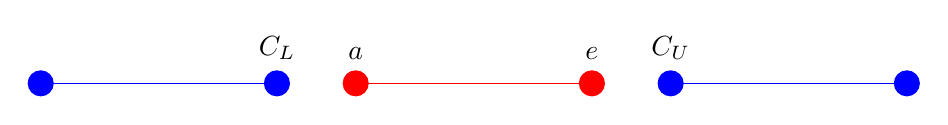
\begin{tikzpicture}[scale=2]
        \coordinate (A) at (0,0);
        \coordinate (B) at (1.5,0);
        \coordinate (C) at (2.0,0);
        \coordinate (D) at (3.5,0);
        \coordinate (E) at (4.0,0);
        \coordinate (F) at (5.5,0);

        \draw[blue] (A) -- (B);
        \draw[red]  (C) -- (D);
        \draw[blue] (E) -- (F);

        \node[circle,fill=blue,radius=0.15]                     at (A) {};
        \node[circle,fill=blue,radius=0.15,label=above : $C_L$] at (B) {};
        \node[circle,fill=red,radius=0.15,label=above  : $a$]   at (C) {};
        \node[circle,fill=red,radius=0.15,label=above  : $e$]   at (D) {};
        \node[circle,fill=blue,radius=0.15,label=above : $C_U$] at (E) {};
        \node[circle,fill=blue,radius=0.15]                     at (F) {};
    \end{tikzpicture}
\end{subfigure}

\par\bigskip

\begin{subfigure}{\textwidth}
    \centering
    \caption{Valid position: $C_L \leq u \leq d \leq e$}
    \label{subfig:all}
    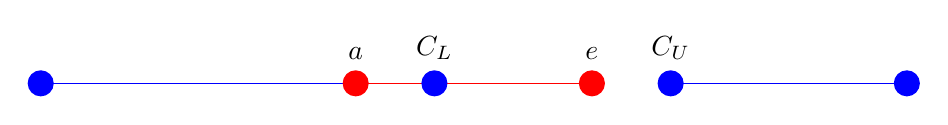
\begin{tikzpicture}[scale=2]
        \coordinate (A) at (0,0);
        \coordinate (B) at (2.5,0);
        \coordinate (C) at (2.0,0);
        \coordinate (D) at (3.5,0);
        \coordinate (E) at (4.0,0);
        \coordinate (F) at (5.5,0);

        \draw[blue] (A) -- (B);
        \draw[red]  (C) -- (D);
        \draw[blue] (E) -- (F);

        \node[circle,fill=blue,radius=0.15]                     at (A) {};
        \node[circle,fill=blue,radius=0.15,label=above : $C_L$] at (B) {};
        \node[circle,fill=red,radius=0.15,label=above  : $a$]   at (C) {};
        \node[circle,fill=red,radius=0.15,label=above  : $e$]   at (D) {};
        \node[circle,fill=blue,radius=0.15,label=above : $C_U$] at (E) {};
        \node[circle,fill=blue,radius=0.15]                     at (F) {};
    \end{tikzpicture}
\end{subfigure}

\par\bigskip

\begin{subfigure}{\textwidth}
    \centering
    \caption{Valid position: $a \leq u \le d \leq C_U$}
    \label{subfig:egu}
    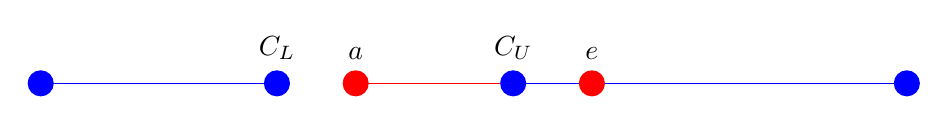
\begin{tikzpicture}[scale=2]
        \coordinate (A) at (0,0);
        \coordinate (B) at (1.5,0);
        \coordinate (C) at (2.0,0);
        \coordinate (D) at (3.5,0);
        \coordinate (E) at (3.0,0);
        \coordinate (F) at (5.5,0);

        \draw[blue] (A) -- (B);
        \draw[red]  (C) -- (D);
        \draw[blue] (E) -- (F);

        \node[circle,fill=blue,radius=0.15]                     at (A) {};
        \node[circle,fill=blue,radius=0.15,label=above : $C_L$] at (B) {};
        \node[circle,fill=red,radius=0.15,label=above  : $a$]   at (C) {};
        \node[circle,fill=red,radius=0.15,label=above  : $e$]   at (D) {};
        \node[circle,fill=blue,radius=0.15,label=above : $C_U$] at (E) {};
        \node[circle,fill=blue,radius=0.15]                     at (F) {};
    \end{tikzpicture}
\end{subfigure}

\par\bigskip

\begin{subfigure}{\textwidth}
    \centering
    \caption{Valid position: $C_L \le u \leq d \leq C_U$}
    \label{subfig:invertsandwhich}
    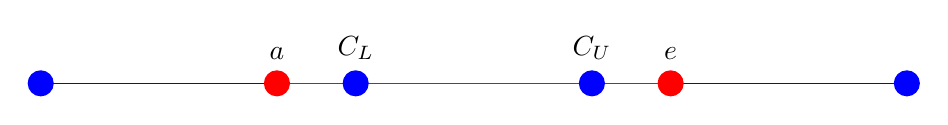
\begin{tikzpicture}[scale=2]
        \coordinate (A) at (0,0);
        \coordinate (B) at (1.5,0);
        \coordinate (C) at (2.0,0);
        \coordinate (D) at (3.5,0);
        \coordinate (E) at (4.0,0);
        \coordinate (F) at (5.5,0);

        \draw[blue] (A) -- (C);
        \draw[blue] (D) -- (F);
        \draw[red]  (B) -- (E);

        \node[circle,fill=blue,radius=0.15]                    at (A) {};
        \node[circle,fill=red,radius=0.15,label=above : $a$]   at (B) {};
        \node[circle,fill=blue,radius=0.15,label=above: $C_L$] at (C) {};
        \node[circle,fill=blue,radius=0.15,label=above: $C_U$] at (D) {};
        \node[circle,fill=red,radius=0.15,label=above : $e$]   at (E) {};
        \node[circle,fill=blue,radius=0.15]                    at (F) {};
    \end{tikzpicture}
\end{subfigure}

\par\bigskip

\begin{subfigure}{\textwidth}
    \centering
    \caption{Invalid position upper bound}
    \label{subfig:invalid-upper}
    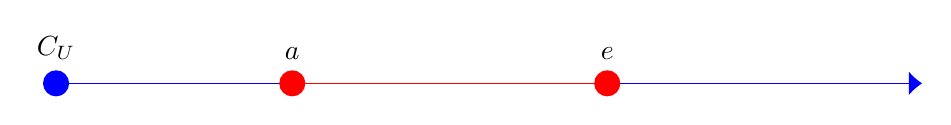
\begin{tikzpicture}[scale=2]
        \coordinate (A) at (0.0,0);
        \coordinate (B) at (5.5,0);
        \coordinate (C) at (1.5,0);
        \coordinate (D) at (3.5,0);

        \draw[-{Latex[width=3mm]},blue]  (A) -- (B);
        \draw[red]  (C) -- (D);

        \node[circle,fill=blue,radius=0.15,label=above : $C_U$] at (A) {};
        \node[circle,fill=red,radius=0.15,label=above  : $a$] at (C) {};
        \node[circle,fill=red,radius=0.15,label=above  : $e$] at (D) {};
    \end{tikzpicture}
\end{subfigure}

\par\bigskip

\begin{subfigure}{\textwidth}
    \centering
    \caption{Invalid position lower bound}
    \label{subfig:invalid-lower}
    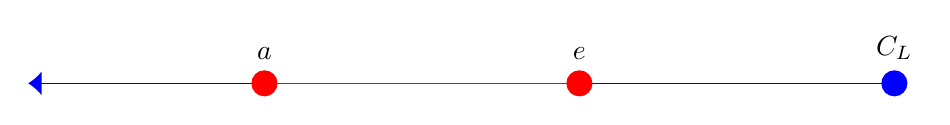
\begin{tikzpicture}[scale=2]
        \coordinate (A) at (0.0,0);
        \coordinate (B) at (5.5,0);
        \coordinate (C) at (1.5,0);
        \coordinate (D) at (3.5,0);

        \draw[-{Latex[width=3mm]},blue]  (B) -- (A);
        \draw[red]  (C) -- (D);

        \node[circle,fill=blue,radius=0.15,label=above : $C_L$] at (B) {};
        \node[circle,fill=red,radius=0.15,label=above  : $a$] at (C) {};
        \node[circle,fill=red,radius=0.15,label=above  : $e$] at (D) {};
    \end{tikzpicture}
\end{subfigure}

\caption{This figure depicts the different states in which a charger with an availability time frame, $[C_L,C_U]$, can be placed on a timeline relative to a visit's total time at the station. The blue lines indicate ranges where the charger is being uilized. The point $C_L$ is the lower bound of the available time and $C_U$ is the upper bound. The red lines, $\bar{ae}$, indicate the time slice in which visit $i$ is at the station. Thus, the BEB may be assigned a charge time anywhere in the range between $C_L$ and $C_U$. For example, \ref{subfig:sandwich} allows the BEB to be charged anywhere in the time range $[a, e]$. \ref{subfig:all} allows a BEB to charge in the time frame $[C_L,e]$. \ref{subfig:egu} allows a BEB to charge in the time frame $[a,C_U]$. \ref{subfig:invertsandwhich} allows charging during the time frame $[C_L,C_U]$. The last two permutations, \ref{subfig:invalid-upper} and \ref{subfig:invalid-lower}, do not allow the BEB to be assigned.}
\label{fig:find-free}
\end{figure}
\begin{algorithm}[H]
\caption{Find free time algorithm checks whether the BEB time at the station, $[a_i, e_i]$ fits within the charger availability $[L,C_U]$. If it does, a random charge time slice is returned, otherwise the null value is returned.}
\label{alg:find-free-time}
    \LinesNumbered
    \TitleOfAlgo{Find Free Time}
    \KwIn{$(\C, i, q, a, e)$}
    \KwOut{($\bar{\C}, \bar{u}, \bar{d})$}

    \Begin
    { \tcc{Extract the lower and upper bounds.}
      $C_L \leftarrow \C_{i.q}$\;
      $C_U \leftarrow \C_{i.q}$\;

      \If(\tcc*[f]{If $C_L \le a \le e \le C_U$ (\autoref{subfig:sandwich})}){$C_L \leq a$ and $C_U \geq e$}
      {
        $\bar{u}\leftarrow$ $\U_{[a,e]}$\;
        $\bar{d}\leftarrow$ $\U_{[\bar{u},e]}$\;
      }
      \ElseIf(\tcc*[f]{Else if $a \le C_L \le e < C_U$ (\autoref{subfig:all})}){$C_L \ge a$ and $C_U \geq e$}
      {
        $\bar{u}\leftarrow$ $\U_{[C_L,e]}$\;
        $\bar{d}\leftarrow$ $\U_{[\bar{u},e]}$\;
      }
      \ElseIf(\tcc*[f]{Else if $C_L \le a \le C_U < e$ (\autoref{subfig:egu})}){$C_L \leq a$ and $C_U \le e$}
      {
        $\bar{u}\leftarrow$ $\U_{[a,C_U]}$\;
        $\bar{d}\leftarrow$ $\U_{[\bar{u},C_U]}$\;
      }
      \ElseIf(\tcc*[f]{Else if $a \leq C_L \leq C_D \leq u$ (\autoref{subfig:invertsandwhich})}){$C_L \ge a$ and $C_U \le e$}
      {
        $\bar{u}\leftarrow$ $\U_{[C_L,C_U]}$\;
        $\bar{d}\leftarrow$ $\U_{[\bar{u},C_U]}$\;
      }
      \Else(\tcc*[f]{Otherwise the bus cannot be scheduled in this time frame (\autoref{subfig:invalid-lower}, \autoref{subfig:invalid-upper})})
      {
        $\bar{u}\leftarrow$ $\varnothing$\;
        $\bar{d}\leftarrow$ $\varnothing$\;
      }

      \If (\tcc*[f]{If an assignment was made}) {$\bar{u},\bar{d} \ne \varnothing$}
      {
        $\bar{\C}_q' \leftarrow \C_q' \cup \{[\bar{u},\bar{d}]\}$\tcc*{Update the compliment of the charger free time slices}
        \Return{($\bar{C},\bar{u},\bar{d}$)}
      }
      \Else(\tcc*[f]{Otherwise the assignment failed})
      {
        \Return{($C,\varnothing, \varnothing$)}
      }
    }
\end{algorithm}

\item Purge
\label{sec:purge}
The purge procedure simply removes a assigned charge time from the set \(\C\). This function, while not a generator,
exists so that other primitives may place the visit back into the schedule without creating duplicate entries in \(\C\).
Line 2 from \ref{alg:purge} updates \(\C\) with the set of visits excluding visit \(i\) from charging queue \(q_i\). Line 3
returns the updated set of charger availability.

\begin{algorithm}[H]
  \caption{Purge algorithm} \label{alg:purge}
    \LinesNumbered
    \TitleOfAlgo{Purge}
    \KwIn{$\Sol$}
    \KwOut{$\bar{\Sol}$}

    \Begin
    {
      $\bar{\C} \leftarrow \C \setminus \C_{i.q_i}$\tcc*{Remove assignment of visit $i$ to charger $q_i$}
      \Return{$(i, \I, \bar{\C})$}\tcc*{Return updated tuple}
    }
  \end{algorithm}

\item Slide visit
\label{slide-visit}
This primitive generator is used for buses that have already been scheduled. Because of the constraint \ref{seq:c8}
there may be some slack to manipulate \([u_i, d_i]\) within the window \([a_i, e_i]\). That is, two new values, \(u_i\) and
\(d_i\) are randomly selected with a uniform distribution that satisfy the constraint \(a_i \leq u_i \leq d_i \leq e_i\). Line 2 from
\ref{alg:slide-visit} purges the visit from the charger availability schedule. Line 4 retrieves the window that was
opened up by purging visit \(i\). Line 4 sets the new charge time frame, \([u_i, d_i]\). Line 5 returns the updated visit
information. If \texttt{findFreeTime} was unsuccessful, then the generator returns a tuple of null values.

\begin{algorithm}[H]
  \caption{Slide Visit Algorithm} \label{alg:slide-visit}
  \LinesNumbered
  \TitleOfAlgo{Slide Visit}
  \KwIn{$\Sol$}
  \KwOut{$\bar{\Sol}$}

    \SetKwFunction{Purge}{Purge}

    \Begin
    {
      $(i, \I, \bar{\C}) \leftarrow$\Purge{$\Sol$}\tcc*{Purge visit $i$ from charger availibility matrix}
      $C \leftarrow \bar{C}_{i.q_i}$\tcc*{Get the time availability of the purged visit}

      \tcc{If there is time available in $C$}
      \If{($\bar{C}, \bar{u}, \bar{d}$) $\leftarrow$ \findFreeTime{$C$, $\Sol_i$, $\I_q$, $\I_{i.a}, \I_{i.e}$} $\not\in \varnothing$}
      {
        \Return{($i, \I, (\I_{i.q_i},\bar{u},\bar{d}),\bar{C}$)}\tcc*[f]{Return updated visit}
      }

        \Return{($\varnothing$)}\tcc*{Return nothing}
    }
  \end{algorithm}

\item New charger
\label{new-charger}
The new charger generator moves a visit \(\I_i\) to a new charging queue while maintaining the same charge time, \([u_i,
d_i]\). Line 2 from \ref{alg:new-charger} purges the visit from the charger availability set. Line 3 randomly selects a
charger queue index, \(q\). Line 4 checks if there is an available time slice \([a_i, e_i]\) for charger \(q\). Line 5 returns
the updated visit data. If \texttt{findFreetime} was unsuccessful, then the generator returns a tuple of null values.

\begin{algorithm}[H]
  \caption{New Charger Algorithm} \label{alg:new-charger} \LinesNumbered \TitleOfAlgo{New Charger} \KwIn{$\Sol$}
  \KwOut{$\bar{\Sol}$}

    \SetKwFunction{Purge}{Purge}

    \Begin
    {
      $(i, \I, \bar{\C}) \leftarrow$\Purge{$\Sol$}\tcc*{Purge visit $i$ from charger availibility matrix}
      $q \leftarrow \mathcal{U}_{Q}$\tcc*{Select a random charging queue with a uniform distribution}

      \If(\tcc*[f]{If there is time available in $C_{q}$}){($\bar{C}, \bar{u}, \bar{d}$) $\leftarrow$ \findFreeTime{$\bar{\C}_{i.q}$, $\Sol_i$, $\I_q$, $\I_{i.a}, \I_{i.e}$} $\not\in \varnothing$}
      {
        \tcc{Return visit, note $u$ and $d$ are the original inital/final charge times.}
        \Return{($i, \I, (q,\I_{i.u}, \I_{i.d}),\bar{\C}$)}
      }

      \Return{($\varnothing$)}\tcc*{Return nothing}
    }
  \end{algorithm}

\item Wait
\label{sec:wait}
The wait generator simply removes a bus from a charger queue and places it in its idle queue, \(q_i \in \{1,...,B\}\).
Line 2 from \ref{alg:wait} purges the visit from the charger availability set. Line 4 updates the complement charger
availability schedule of the wait queue for bus \(b\). Line 5 returns the updated visit.

\begin{algorithm}[H]
\caption{Wait algorithm} \label{alg:wait}
    \LinesNumbered
    \TitleOfAlgo{Wait}
    \KwIn{$\Sol$}
    \KwOut{$\bar{\Sol}$}

    \SetKwFunction{Purge}{Purge}

    \Begin
    {
      $(i, \I, \bar{\C}) \leftarrow$\Purge{$\Sol$}\tcc*{Purge visit $i$ from charger availibility matrix}
      $\bar{\C}'_{\I_{i.\Gamma_i}} \leftarrow \C' \cup \{[\I_{i.a}, \I_{i.e}]\}$\tcc*{Update the charger availability matrix for wait queue $\bar{\C}_{i.q_i}$}
      \Return{$(i, \I, (\I_{i.b}, \I_{i.a}, \I_{i.e}), \bar{\C})$}\tcc*[f]{Return visit}
    }
  \end{algorithm}

\item New Window
\label{sec:new-window}
New window, as shown in \ref{alg:new-window}, is a combination of \ref{alg:new-visit} (new visit) and \ref{alg:wait}
(wait). By this it is meant that visit \(i\) is placed in its wait queue then added back in as if it were a new visit.
This implies that the BEB may be assigned to a different queue and a new charge time slice. Line 2 purges the BEB visit
from the schedule producing \(\bar{\Sol}\). Line 3 places the BEB back into the schedule using the new visit generator,
producing \(\bar{\bar{\Sol}}\). Line 4 assigns and returns the updated visit. Line 6 returns the null visit upon failure
of \ref{alg:new-visit}.

\begin{algorithm}[H]
  \caption{New window algorithm} \label{alg:new-window}
  \LinesNumbered
  \TitleOfAlgo{New Window}
  \KwIn{$\Sol$}
  \KwOut{$\bar{\Sol}$}

  \SetKwFunction{NewVisit}{NewVisit}
  \SetKwFunction{Purge}{Purge}

  \Begin
  {
    $\bar{\Sol} \leftarrow$\Purge{$\Sol$}\tcc*{Purge visit $i$ from charger availibility matrix}
    \If(\tcc*[f]{Add visit $i$ back in randomly})
       {
         $\bar{\bar{\Sol}} \leftarrow$ \NewVisit{$\bar{\Sol}$} $\not\in \varnothing$
       }
       {
         \Return{$\bar{\bar{\Sol}}$} \tcc*[f]{Return visit}
       }

       \Return{($\varnothing$)}\tcc*{Return nothing}
  }
\end{algorithm}
\end{enumerate}

\paragraph{Generator Wrappers}
\label{sec:generator-wrappers}
This section covers the algorithms utilized to select and execute different generation processes. The generator wrappers
are the methods immediately called by the SA algorithm. Each wrapper utilizes the primitive generators previously
described and returns either a new charge schedule or a modified charge schedule.

\begin{enumerate}
\item Charge Schedule Generation
\label{sec:charge-schedule-generation}
The objective of \ref{alg:charge-schedule-generation} is to assign each BEB to a random charge queue and charge time.
Specifically, this generator exists to initialize the system with a solution in a greedy manner. Line 2 of
\ref{alg:charge-schedule-generation} loops through each visit and Line 4 executes \ref{alg:new-visit} to place visit \(i\)
at random queue with a random charge time.

\begin{algorithm}[H]
\caption{Charge schedule generation algorithm} \label{alg:charge-schedule-generation}
    \LinesNumbered
    \TitleOfAlgo{Candidate Solution Generator}
    \KwIn{$\Sol$}
    \KwOut{$\bar{\Sol}$}

    \SetKwFunction{NewVisit}{NewVisit}

    \Begin
    {
        \tcc{Select an unscheduled BEB visit from a randomly indexed set of visits}
        \ForEach {$\I_i \in \I$}
        {
            ($i, \bar{\I}$, $\bar{\C}$) $\leftarrow$ \NewVisit{($\I_i$, $\I$, $\C$)}\tcc*{Assign the bus to a charger}
        }
            \Return{($0, \bar{\I}$, $\bar{\C}$)}
    }
  \end{algorithm}

\item Perturb Schedule
\label{sec:tweak-schedule}
Once the active solution has been created by \ref{alg:charge-schedule-generation}, the SA process begins modifying it to
create candidate solutions. After each step of the cooling function, the active solution will be altered \(n_K\) times by
a random primitive generator. During these \(n_K\) iterations the active solution is modified to create a neighboring
candidate solution. This candidate solution will then be compared against the active solution in the manner discussed in
\ref{sec:acceptance}. \ref{alg:perturb-schedule} describes the method by which the SA algorithm decides how to perturb the
schedule. The method that will be employed generate a neighboring solution is as follows: pick a visit, pick a primitive
generator, and execute said primitive generator once. Furthermore, the primitives are not desired to be picked at random
with a uniform distribution. That is, a weighted distribution is required. Let \(\W^y_{[\cdot]}\) denote a random selection
with a distribution specified by a weight vector \(y \in \mathbb{R}\). Thus, \ref{alg:perturb-schedule} is as follows: Line 2 selects
a visit at random with a uniform distribution. Line 3 extracts the visit index and Line 4 creates a vector of weights
associated with a primitive generator. Letting \(n_G\) denote the number of primitive generating functions, Line 5 selects
a primitive generator with a weighted distribution. Line 6 executes the primitive, and Line 7 returns the result.

\begin{algorithm}[H]
\caption{Perturb schedule algorithm} \label{alg:perturb-schedule}

    \LinesNumbered
    \TitleOfAlgo{Perturb Schedule}
    \KwIn{$\Sol$}
    \KwOut{$\bar{\Sol}$}

    \SetKwFunction{PGF}{PGF}

    \Begin
    {
        $\I_i\leftarrow\; \U_{\I}$\tcc*{Randomly select a visit}
        $i \leftarrow\; \I_i$\tcc*{Extract visit index}
        $y \leftarrow [y_1, y_2, ...]$\tcc*{Define the weight of each primitive generator}
        $PGF \leftarrow\; \W^y_{[1,n_G]}$\tcc*{Select one of the generator functions}
        $\bar{\Sol} \leftarrow$ \PGF{($i$, $\I$, $\C$)}\tcc*{Excecute the generator function}
        \Return{($0, \bar{\I}$, $\bar{\C}$)}
    }
\end{algorithm}
\end{enumerate}

\subsubsection{Alternative Heuristic Implementation}
\label{sec:heuristic-implementation}
As suggested by the works in \cite{Zhang_2010,Xinchao_2011}, applying heuristics to the generating functions can
manipulate the searched neighborhoods in a way that may assist the SA algorithm with convergence. As a test to assist in
minimizing charger utilization, a simple heuristic was applied to \ref{alg:new-visit} and \ref{alg:new-charger} in the
method that they select new charging queues. Suppose rather than selecting a queue at random from \(q \in Q\), the
algorithms randomly select whether to place a BEB in a slow or fast charging queue with a weighted distribution favoring
slow chargers. Once the charger type has been selected, the algorithm will then begin incrementally attempting to place
the BEB in a queue of that type beginning from the smallest index of that charger type. For example, if a BEB has been
selected to be placed in a queue with a slow charger, the algorithm begins by attempting to place the BEB in the charger
queue \(q = n_B + 1\). If it is unable to be placed in that queue, it then attempts to be placed in the next queue \(q =
n_B + 2\). This is done incrementally until all the queues have been exhausted.

\subsection{Optimization Algorithm}
\label{sec:optimization-algorithm}
This section combines the generation algorithms and the optimization problem into a single algorithm. It begins with an
introduction and discussion of a general SA algorithm which will be used to springboard into the construction of the SA
PAP algorithm.

\subsubsection{Simulated Annealing Pseudo Code}
\label{sec:simulated-annealing-pseudo-code}
Let \(\omega\) and \(\bar{\omega}\) denote the active solution and the candidate solution, respectively. Let \(\Tau\) be the temperature
function and \(\Tau_0\) the initial temperature. Furthermore, let \(t\) be defined as the vector of temperatures defined by
\(t = \Tau(\Tau_0)\), and let \(t_m\) be defined as being an element of \(t\), \(t_m \in t\). Let \(n_K\) be the repetition counter,
it defines the number of iterations to execute exploit a solution at a constant temperature \(t_m\).

Recall the objective of the SA algorithm is to iteratively create a neighboring candidate solution from the active
solution. The fitness of the two solutions are compared and if the candidate solution is of a higher quality, it is
always taken as the active solution. If it is not, then it may be selected as the new candidate solution with some
probability that is a function of the difference in the objective function values and the current temperature. This
process is iteratively done until the temperature function reaches its minimum value. With the high level summary in
mind, the SA pseudocode is to be presented \cite{henderson-1989-theor-pract}.

The algorithm behaves as follows: Lines 1 and 2 of \ref{alg:sa-pseudo} initialize the SA algorithm the temperature
schedule, \(t\), and active solution, \(\omega\), respectively. The outer loop on Line 3 iterates through all the temperature
values in \(t\). After each iteration of the outer loop, the temperature is decreased as specified by the selected
temperature function. Line 4 resets the iteration counter to 0. Line 5 specifies the inner loop that iterates \(n_K\)
times at a constant temperature, \(t_k\). Line 6, perturbs the active solution \(\omega\) to a neighboring candidate solution
\(\bar{\omega} = N(\omega)\). Line 7 then calculates the difference in the fitness of \(\omega\) and \(\bar{\omega}\). Lines 8-13 updates \(\omega\) with
\(\bar{\omega}\) if the candidate solution is more fit, or updates \(\omega\) with \(\bar{\omega}\) with probability \(e^{\frac{-\Delta_{\omega ,
\bar{\omega}}}{t_m}}\) if the candidate solution is less fit than the active solution. Line 14 updates the repetition counter.

\begin{algorithm}[H]
\caption{Pseudo-code for SA} \label{alg:sa-pseudo}
    \LinesNumbered
    \TitleOfAlgo{SA Pseudo-Code}

    \SetKwFunction{Obj}{J}
    \SetKwFunction{New}{N}
    \SetKwFunction{Pert}{P}
    \SetKwFunction{Temp}{$\Tau$}

    \Begin
    {
        \tcc{Generate vector of temperatures given temperature function $\Tau$ and initial temperature $\Tau_0$}
        $t \leftarrow$ \Temp{$\Tau_0$}\;
        $\omega \leftarrow$ \New{($\I$, $\C$)}\tcc*{Generate an initial solution}

        \ForEach{$t_m \in t$}
        {
          $k \leftarrow 0$ \tcc*{Initialize repetition counter}

          \ForEach{$k \in \{0, 1, ..., n_K$}
          {
            $\bar{\omega} \leftarrow $ \Pert{($\I$, $\C$)}\tcc*{Perturb the solution}
            $\Omega_{\bar{\omega},\omega} \rightarrow$ \Obj{$\bar{\omega}$} - \Obj{$\omega$}\tcc*{Calculate the difference of fitness scores}

            \tcc{Compare and update current solution}
            \If{$\Omega_{\bar{\omega},\omega} \le 0$}{$\omega \leftarrow \bar{\omega}$}
            \If{$\Omega_{\bar{\omega},\omega} > 0$}{$\omega \leftarrow \bar{\omega}$ with probability $e^{\frac{-\Omega_{\bar{\omega},\omega}}{t_m}}$}
          }
        }
    }
\end{algorithm}

\subsubsection{SA PAP Pseudo Code}
\label{sec:sa-pap-pseudo-code}
Now that the general SA algorithm has been outlined, the objective is now to outline SA-PAP (\ref{alg:sa-pap}). While
the SA PAP generally is written almost identically to that of the general SA algorithm, the general SA assumes that the
generated candidate solutions are in the solution space of the problem, \(\omega \in S\) where \(S\) is the solution space.
Initialization and the perturbation of a schedule must be verified to ensure that the generated schedule is in the
solution space. Therefore, the objective function and constraints introduced in \ref{sec:constraints} and
\ref{sec:objective-function}, respectively, must be employed to verify that the output of
\ref{alg:charge-schedule-generation} is in the feasible space, \(S\).

As previously stated, the generating functions directly influence the values of the assigned charge queue, charge
initialization time, and charge completion time: \(q_i\), \(u_i\), and \(d_i\), respectively. Having generated those values,
the rest of the decision variables may be derived. Let's begin by reviewing over the packing constraints.
\ref{seq:c0}-\ref{seq:c1} are employed to enable and disable \(\sigma_{ij}\) and \(\psi_{ij}\) and \ref{seq:c2}-\ref{seq:c4} ensure
the validity of the values. \ref{seq:c5} can be directly calculated and \ref{seq:c8} is fully defined.

Changing the focus over to the dynamic constraints, similarly to what was seen with the packing constraints, the battery
dynamic constraints are also fully defined and can be calculated. \ref{seq:c6} is sequentially calculated after a given
schedule has been fully defined. \ref{seq:c7} is evaluated to ensure the BEB is not overcharged. The penalty method
implemented in \ref{sec:objective-function} is set in place to allow the SOC to go below the specified threshold, \(\nu_{\Xi_i}
\kappa_{\Xi_i}\), but punish the solution for doing so. Thus, over time, the candidate solutions will be encouraged toward a
solution that does not activate the penalty method (i.e. is solution is truly feasible).

The SA-PAP algorithm in \ref{alg:sa-pap} will now be outlined. Line 2 initializes the SA algorithm by creating a vector
of temperature values based on a temperature schedule \(\Tau\), and initial temperature \(\Tau_0\). Line 3 generates the
initial candidate solution \(\omega\), note that \(CSG(\cdot)\) (candidate solution generator) is used to denote the specific
candidate solution generator being utilized. For SA PAP it is \ref{alg:charge-schedule-generation}. Line 4 loops through
each of the step in the temperature schedule \(t_m \in t\). Line 5 resets the iteration count to 0. Line 6 specifies the
inner loop that iterates \(n_K\) times at a constant temperature, \(t_k\). Line 7, perturbs the active solution \(\omega\) to a
neighboring candidate solution \(\bar{\omega} = PS(\omega)\), where \(PS(\cdot)\) (perturb schedule) is \ref{alg:perturb-schedule}. Line 8
calculates the difference in the fitness of \(\omega\) and \(\bar{\omega}\). Lines 8-14 are similar to \ref{alg:sa-pseudo} where it
updates \(\omega\) with \(\bar{\omega}\) if the candidate solution is more fit, or updates \(\omega\) with \(\bar{\omega}\) with probability
\(e^{\frac{-\Delta_{\bar{\omega},\omega}}{t_m}}\) if the candidate solution is less fit than the active solution. What makes these lines
unique is that the active solution is only updated if the candidate is within the solution space. That it, it satisfies
the constraints defined in \ref{eq:constraints}.

\begin{algorithm}[H]
  \caption{Simulated annealing approach to the position allocation problem} \label{alg:sa-pap}
  \LinesNumbered
  \TitleOfAlgo{SA PAP}
  \KwIn{($\I$ , $\C$)}
  \KwOut{($\bar{\I}$, $\bar{\C}$)}

  \SetKwFunction{Temp}{$\Tau$}
  \SetKwFunction{CSG}{CSG}
  \SetKwFunction{PS}{PS}
  \SetKwFunction{Obj}{J}

  \Begin
    {
      \tcc{Generate vector of temperatures given temperature function $\Tau$ and initial temperature $\Tau_0$}
      $t \leftarrow$ \Temp{$\Tau_0$}

      $\omega \leftarrow$\CSG{($\I$, $\C$)}\tcc{Generate an initial solution}

      \tcc{For each item in the temperature vector}
      \ForEach{$t_k \in t$}
       {
         $k \leftarrow 0$\tcc*{Initialize repetition counter}

        \tcc{For each step in the repitition schedule}
        \ForEach{$t_m \in t$}
        {
          $\bar{\omega} \leftarrow$ \PS{($\I$, $\C$)} \tcc*{Generate a new solution}
          $\Omega_{\bar{\omega},\omega} = $ \Obj{$\bar{\omega}$}  - \Obj{$\omega$} \tcc*{Calculate the difference of fitness scores}

          \If{$\bar{\I} \in S$ and $\Omega_{\bar{\omega},\omega} \le 0$}{$\omega \leftarrow \bar{\omega}$}
          \If{$\bar{\I} \in S$ and $\Omega_{\bar{\omega},\omega} > 0$}{$\omega \leftarrow \bar{\omega}$ with probability $e^{\frac{\Omega_{\omega, \bar{\omega}}}{t_k}}$}
        } % For k
      }   % For t_k \in t

      \Return{($\bar{\I}$ , $\bar{\C}$)}
    } % Begin
\end{algorithm}

\section{Summary}
\label{sec:approach-summary}
The previous sections discussed the approaches to be taken (or have taken) for each respective objective along with a
derivation when available for the proposed approach. A projected project schedule was also provided. This research
intends to increase utility of the PAP by first modifying the model to allow BEBs' charges to be propagated, include an
identifier for BEBs to be tracked, utilize non-linear charging dynamics, as well as utilizing FFLP to develop a robust
solution. Upon completion, the proposed research will demonstrate its full utility and extensibility due to the MILP's
nature of adding additional constraints. This research project shall illustrate a robust BEB charging schedule with
realistic applicability.

\references{citation-database/lib-ref,citation-database/lit-ref}{IEEEtran}
\end{document}
